\documentclass[12pt,a4paper,twoside]{book}
\usepackage{graphicx}
\usepackage{setspace}	%double spacing for text, single for captions, footnotes, etc.
%\usepackage{hypernat} 	%substitut de cite que permet fer hyperlinks
\usepackage{natbib}		% substituye a 'hypernat' que funciona en Windows.
\usepackage[spanish]{babel}
\usepackage[utf8]{inputenc}
\usepackage{color}
\usepackage{hhline} 		% extended styles for tables
\usepackage{multirow}
\usepackage{subfigure}
\usepackage{acronym}
\usepackage{hyperref}
\usepackage{amsmath,amsmath,amssymb} 
\usepackage{fancyhdr}
\usepackage{epsfig, amsmath}
\usepackage{algorithm}
\usepackage{algorithmic}
\usepackage{epigraph}
\usepackage{titlesec}
\usepackage{amsmath}


% general settings
\hypersetup{
	linktocpage=true,
	colorlinks=true,
	linkcolor=blue,
	citecolor=blue,
}
\definecolor{Hgray}{gray}{0.6}

\newenvironment{definition}[1][Definition]{\begin{trivlist}
\item[\hskip \labelsep {\bfseries #1}]}{\end{trivlist}}

\setlength{\topmargin}{0cm}
\setlength{\textheight}{23cm}
\setlength{\textwidth}{17cm}
\setlength{\oddsidemargin}{0cm}
\setlength{\evensidemargin}{0cm}
\setlength{\headheight}{1cm}
\setlength{\parskip}{0.5cm}

% indica que las 'sub-sub-sections' sean numeradas y aparezcan en el indice
\setcounter{secnumdepth}{3}
\setcounter{tocdepth}{2}

% settings for code
\renewcommand{\algorithmicrequire}{\textbf{Entrada: }}
\renewcommand{\algorithmicensure}{\textbf{Salida: }}
%\newcommand{\sectionbreak}{\clearpage}

%%%%%%%%%%%%
% DOCUMENT %
%%%%%%%%%%%%
\begin{document}

% portada
\newpage
\thispagestyle{empty}

\baselineskip 2em

%\vspace*{1cm}

\centerline{
\includegraphics[width=0.6\textwidth]{images/UOC-logo}}
\begin{center}
\textsc{Universitat Oberta de Catalunya (UOC) \\
 Máster Universitario en Ciencia de Datos (\textit{Data Science})\\}

%\centerline {\pic{UOC}{4cm}}

\vspace*{1.5cm}

\textsc{\Large TRABAJO FINAL DE MÁSTER}

\vspace*{0.5cm}

\textsc{\large Área: Minería de datos y Machine Learning}


%\textbf{\Huge VirtualTechLab Model: }

\vspace*{2.0cm}

\textbf{\Large Detección de anomalías en entorno del Internet de las cosas}


\vspace{2.5cm}
\baselineskip 1em

\baselineskip 2em
-----------------------------------------------------------------------------\\
Autor:      Gonzalo Pedro Mellizo-Soto Díaz\\
Tutor:      Carlos Hernández Gañán \\
Profesor:   Jordi Casas Roma \\
-----------------------------------------------------------------------------\\
\vspace*{1.5cm}
Madrid, \today

\end{center}

\newpage
\pagestyle{empty}
\hfill

\newpage
% abstract
\pagenumbering{roman} 
\setcounter{page}{1} 
\pagestyle{plain}

%%%%%%%%%%%%%%%%
%%% CREDITOS %%%
%%%%%%%%%%%%%%%%
\chapter*{Copyright}

\vspace{1cm}

\begin{figure}[ht]
    \centering
	
\includegraphics[scale=1]{images/license.png}
\end{figure}

Esta obra está sujeta a una licencia de Reconocimiento -  NoComercial - SinObraDerivada

\href{https://creativecommons.org/licenses/by-nc-nd/3.0/es/}{3.0 España de CreativeCommons}.

%%%%%%%%%%%%%
%%% FICHA %%%
%%%%%%%%%%%%%
\chapter*{FICHA DEL TRABAJO FINAL}

\begin{table}[ht]
	\centering{}
	\renewcommand{\arraystretch}{2}
	\begin{tabular}{r | l}
		\hline
		Título del trabajo: & Detección de anomalías en el entorno del Internet de las cosas\\
		\hline
        Nombre del autor: & Gonzalo Pedro Mellizo-Soto Díaz\\
		\hline
        Nombre del colaborador/a docente: & Carlos Hernández Gañán\\
		\hline
        Nombre del PRA: & Jordi Casas Roma\\
		\hline
        Fecha de entrega (mm/aaaa): & 06/2019\\
		\hline
        Titulación o programa: & Máster Universitario en Ciencia de Datos\\
		\hline
        Área del Trabajo Final: & Minería de datos y Machine Learning \\
		\hline
        Idioma del trabajo: & Español\\
		\hline
        Palabras clave & Machine Learning, IOT, Anomaly Detection\\
		\hline
	\end{tabular}
\end{table}

%%%%%%%%%%%%%%%%%%%
%%% DEDICATORIA %%%
%%%%%%%%%%%%%%%%%%%
\chapter*{Cita}

\setlength\epigraphwidth{.8\textwidth}
\setlength\epigraphrule{0pt}

\epigraph{\itshape``Nuestro lema es: más humanos que los humanos"}{Eldon Tyrell, \textit{Blade Runner}}

%%%%%%%%%%%%%%%%%%%
%%% Agradecimientos %%%
%%%%%%%%%%%%%%%%%%%
\chapter*{Agradecimientos}

TO BE DEFINED

Si se considera oportuno, mencionar a las personas, empresas o instituciones que hayan contribuido en la realización de este proyecto.

%%%%%%%%%%%%%%%%
%%% RESUMEN  %%%
%%%%%%%%%%%%%%%%
\chapter*{Abstract}
\addcontentsline{toc}{chapter}{Abstract}

\onehalfspacing

In recent years the amount of connected devices has greatly increased, with an increasing number of applications in the industry each day. This devices can be subject of attacks causing instability or data leaks that can be dangerous both for the users and the enterprises, in order to avoid or confront them, security and early detection are becoming a must in a connected world. The focus is the monitoring and detection of the attacks in Internet of Things devices using state of the art Machine Learning techniques. Models such as SVM, DBScan or Isolation Forests have been used and assembled in order to identify with a better accuracy when an attack is happening. With this assembly, attack detection has increased up to 15\% comparing to traditional methods and individual model usages and times have been considerably reduced. An active use of Machine Learning models has shown a great improvement at anomaly detection by securing the devices and decreasing the reaction times when facing attacks.

\vspace{0.5cm}

Durante los últimos años se encuentra una creciente cantidad de dispositivos conectados entre sí, cada vez con más aplicaciones en la industria. Estos dispositivos pueden ser atacados y provocar inestabilidad o una fuga de datos, por lo tanto la protección y la pronta detección de ataques y/o anomalías es vital en un mundo cada vez más conectado. El objetivo es la monitorización y detección de estos ataques en dispositivos del \textit{Internet of Things} utilizando técnicas del estado del arte de Machine Learning para su detección y poder así responder con una mayor rapidez a los ataques. Para la detección se han utilizado modelos estadísticos, como SVM, DBScan o Isolation Forests, que en su conjunto permitan identificar con mayor precisión cuando se está produciendo un ataque. El conjunto de la clusterización con la clasificación de puntos anómalos muestra una mayor robustez, frente al uso individual de cada uno de los modelos aumentando la detección en hasta un 15\%. Se demuestra cómo el uso de los modelos permite proteger los dispositivos y mejorar la seguridad al disminuir los tiempos de reacción frente a los ataques.

\vspace{0.5cm}
\textbf{Palabras clave}: Machine Learning, IOT, Anomaly Detection
\newpage

\pagestyle{fancy}
\renewcommand{\chaptermark}[1]{ \markboth{#1}{}}
\renewcommand{\sectionmark}[1]{\markright{ \thesection.\ #1}}
\lhead[\fancyplain{}{\bfseries\thepage}]{\fancyplain{}{\bfseries\rightmark}}
\rhead[\fancyplain{}{\bfseries\leftmark}]{\fancyplain{}{\bfseries\thepage}}
\cfoot{}

% indice
\cleardoublepage
\phantomsection
\addcontentsline{toc}{chapter}{Índice}
\tableofcontents
% listado de figuras
\cleardoublepage
\phantomsection
\addcontentsline{toc}{chapter}{Listado de Figuras}
\listoffigures
% listado de tablas
\cleardoublepage
\phantomsection
\addcontentsline{toc}{chapter}{Listado de Tablas}
\listoftables

\thispagestyle{empty}

\pagenumbering{arabic}

\pagestyle{fancy}
\renewcommand{\chaptermark}[1]{ \markboth{#1}{}}
\renewcommand{\sectionmark}[1]{\markright{ \thesection.\ #1}}
\lhead[\fancyplain{}{\bfseries\thepage}]{\fancyplain{}{\bfseries\rightmark}}
\rhead[\fancyplain{}{\bfseries\leftmark}]{\fancyplain{}{\bfseries\thepage}}
\cfoot{}

\onehalfspacing

% capitulos del documento
\chapter{Introducción}
\label{chapter:introduccion}


%%% SECTION
\section{Contexto y justificación del Trabajo}
Cada vez se encuentran más dispositivos conectados entre sí no solo en la industria, si no también en los hogares, esta conexión entre dispositivos los hace vulnerables a ataques informáticos que pueden afectar en gran medida a los usuarios, no solo pueden provocar un mal funcionamiento de los mismos, si no que también puede provocar la fuga de datos de distinta sensibilidad. La previsión en los futuros años es de cada vez estar más conectados y una pronta detección de los ataques puedo ayudar a evitar los problemas derivados de los mismos, mediante una pronta reacción o frente a la previsión de un ataque.

\vspace{0.5cm}

Actualmente se utilizan distintas medidas de seguridad como control de acceso físico al dispositivo, encriptación de datos, firewalls, securización de red, etc... Sin embargo, en muchos casos la detección de anomalías aplican un umbral estacionario, provocando que en el caso de un ataque ya sea demasiado tarde para reaccionar o no sean capaz de identificar patrones extraños previos al ataque. Con la aplicación de nuevas técnicas se pretende mejorar los tiempos de reacción e incluso predecir cuándo puede suceder un ataque.

\section{Explicación de la motivación personal}
La razón principal de la selección del proyecto es la posibilidad de aprender y utilizar técnicas de Machine Learning en un sector desconocido que permita diversificar conocimientos. Cada vez más todo se encuentra conectado e investigar cómo clasificar cuando se está produciendo un ataque permite profundizar en conocimientos de seguridad y aplicarlos en un problema real.

\vspace{0.5cm}

La aplicación de técnicas en un problema real ayuda a comprender mejor el uso de las herramientas y el por qué y cuándo se deben de utilizar. De este modo, se añade un nuevo conocimiento que puede aportar en el ámbito profesional y puede utilizarse también en un entorno privado.


\section{Objetivos del Trabajo}
Los objetivos del trabajo son los siguientes:

\begin{itemize}
  \item Adquisición de conocimiento del sector y de los dispositivos IOT
  \item Lectura y comprensión de las técnicas del estado del arte en detección de anomalías en dispositivos conectados.
  \item Obtención de datos reales de conexiones a dispositivos IOT, en caso de no ser posible, generación de datos sintéticos.
  \item Prueba de las técnicas encontradas y evaluación en el problema actual.
  \item Investigación de algoritmos tradicionales de Machine Learning y su utilidad en el problema actual.
  \item Desarrollo de la solución utilizando los algoritmos más aptos.
  \item Evaluación de la detección de patrones y ataques de las técnicas utilizadas.
  \item Comparar los resultados obtenidos con el estado del arte y probar si existen mejoras frente a los métodos actuales.
\end{itemize}

\section{Descripción general del problema}

En la actualidad, la cantidad de dispositivos informáticos existentes que pueden ser víctimas de un ataques es masiva, por lo que securizar bien los dispositivos es fundamental. A pesar de el uso de distintos protocolos de seguridad, se generan nuevos tipos de ataque todos los días, por lo tanto la detección es una necesidad para evitar los problemas derivados.

\vspace{0.5cm}

La pérdida de control de los dispositivos o la fuga de información de los mismos puede provocar pérdidas millonarias a las empresas o provocar una gran inseguridad a los usuarios de productos IOT, así como provocar posibles daño a infraestructuras o personas. Por otro lado, muchos de los dispositivos pueden no tener la capacidad de computación necesaria para incluir una capa de seguridad robusta, que puede compensarse con una detección temprana. 


\section{Enfoque y método seguido}
El enfoque es aplicado al conocer el problema y se intenta dar respuesta a preguntas específicas, mediante la aplicación de los conocimientos obtenidos y la evaluación de la propia aplicación de los mismos.  \par

\vspace{0.5cm}

El método seguido del desarrollo se va a implementar dentro del marco de trabajo \textit{Agile} pensando el desarrollo de la solución como un producto, de este modo se podrá iterar sobre una arquitectura definida y enfocarse en el desarrollo del producto en su total, frente a un modelo tradicional de cascada donde cada fase de desarrollo recae en una sola parte del total.

\vspace{0.5cm}

El formato de entrega será mediante un \textit{minimum viable product} (MVP) en sprints de dos semanas durante el periodo de desarrollo y evaluación de las necesidades según la evolución del producto.

\section{Planificación del Trabajo}

Para la planificación del trabajo se han subdividido las tareas principales y se han mostrado en el siguiente diagrama de Gantt \ref{fig:gantt}.

\begin{itemize}
    \item Pec01 - Definición
    \item Pec01 - Planificación
    \item Pec02 - Búsqueda de fuentes del estado del arte
    \item Pec02 - Lectura de estado del arte
    \item Pec02 - Justificación de estado del arte
    \item Pec02 - Redacción
    \item Pec02 - Refinamiento de objetivos
    \item Pec03 - Planificación de Sprints
    \item Pec03 - Sprint 1
    \item Pec03 - Sprint 2
    \item Pec03 - Sprint 3
    \item Pec03 - Refinamiento/Redacción
    \item Pec04 - Revisión apartados anteriores
    \item Pec04 - Redacción nuevos apartados
    \item Pec05 - Presentación y defensa
\end{itemize}



\begin{figure}[h]
	\centering
	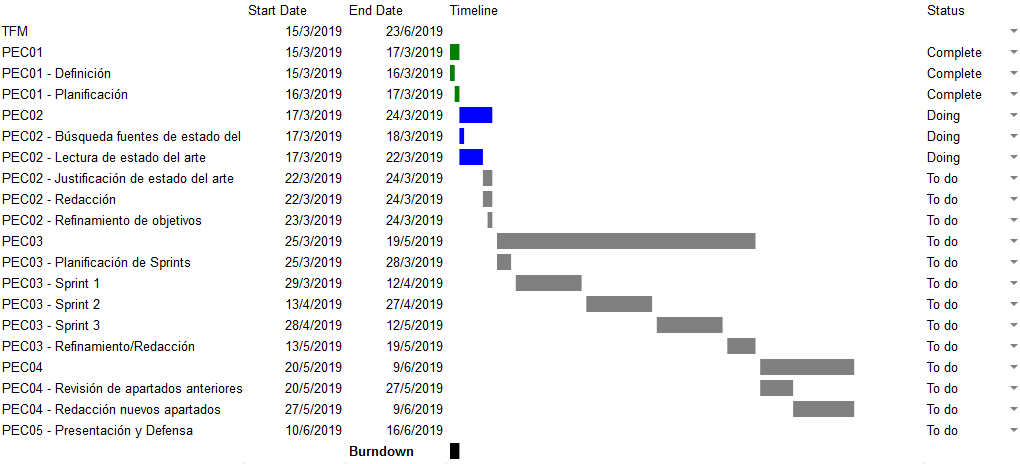
\includegraphics[width=1\textwidth]{figs/gantt_init.PNG}
	\caption{Planificación de tareas}
	\label{fig:gantt}
\end{figure}

\newpage
\chapter{Estado del Arte}
\label{chapter:Estado del Arte}

Una de las aplicaciones más comunes dentro de la detección de anomalías es para la detección de intrusos (\textit{Intrusion Detection}) y la creación de sistemas de detección de intrusos (\textit{Intrusion Detection System, IDS}). Se trata de sistemas cuyo objetivo es la monitorización de los sistemas y redes informáticas, con el fin de alertar en caso de que puedan existir brechas de seguridad\cite{intrusionSystems}. 

Con la ingente cantidad de redes y sistemas que se pueden encontrar a día de hoy es necesario incluir uno de estos sistemas, con el fin de mantener la integridad y disponibilidad de los mismos. Dentro de los IDS, se pueden identificar dos grandes implementaciones de estos sistemas, en los sistemas de detección de intrusos en Host (\textit{Host-Based Intrusion Detection Systems, HIDS}) y los sistemas de detección de intrusos en red (\textit{Network Intrusion Detection Systems, NIDS}).

\begin{itemize}
    \item \textbf{HIDS:} Estos sistemas se caracterizan por implementarse en el Host utilizando información del propio sistema operativo para detectar actos maliciosos \cite{HIDS}. Esta información tiene distintos niveles de información, pero por lo general tienden a ser de bajo nivel sobre operaciones que se pueden estar realizando dentro del sistema. Esta información se consulta dentro de logs, por lo que el análisis de la información es más lento.
   \item \textbf{NIDS:} Para el segundo caso la monitorización se realiza a sistema de red, es decir, de comunicaciones entre distintos nodos y la monitorización de los paquetes que viajan entre ellos \cite{intrusionSystems}. Esta información puede ser consumida en tiempo real, por lo que la reacción ante algún evento es más rápida que en los HIDS que necesitan revisar las acciones.
\end{itemize}

%%% SECTION
\section{Métodos tradicionales de detección de anomalías}
En la sección actual se describen algunos de los métodos tradicionales utilizados en IDS, tanto para HIDS como para NIDS.

\begin{itemize}
    \item Network Security Monitor (NSM):  se trata de uno de los primeros sistemas que permitió auditar el tráfico que circulaba dentro de la red \cite{surveyIDS}. El sistema escucha pasivamente dentro de la red y detecta si existe una conducta sospechosa al desviarse de patrones de conducta. La mayor parte de la monitorización se basa en protocolos estándar como \textit{telnet, ftp, TCP/IP, etc.} por lo que le permitía utilizar una gran cantidad de datos heterogéneos.
    \item State transition analysis (USTAT): el sistema parte de que el host en un momento se encuentra en un estado seguro y que según las acciones que se realizan sobre el mismo el host cambia de estado, hasta que llega a un estado en el que compromete la seguridad \cite{surveyIDS}. Este sistema analiza los estados por los que ha pasado la máquina desde el estado seguro al comprometido. 
    \item GrIDS: se trata de un IDS que utiliza un sistema de construcción de grafos basados en la red, donde cada nodo representa a un host y las aristas las conexiones entre los mismos. La representación gráfica de la actividad de la red permite ayudar al espectador en identificar qué está sucediendo \cite{surveyIDS}.
    \item Haystack: en este caso el IDS se ayuda de métodos estadísticos para la detección de anomalías, definiendo estrategias para usuarios y grupos, además de definir variables del modelo como variables gaussianas independientes \cite{garcia2009anomaly}. Para la detección se incluyen una serie de intervalos en los valores que en el momento que salen del rango normal, se calcula la distribución de probabilidades y si el \textit{score} o puntuación es demasiado grande se genera una alerta.
\end{itemize}

Los métodos/sistemas listados se desarrollaron durante los años noventa, la tecnología ha evolucionado desde entonces y los sistemas se han vuelto más complejos y más propensos a los ciberataques. Por ello, se han desarrollado nuevas técnicas que se apoyan en el uso de técnicas de minería de datos (\textit{Data Mining}) y las técnicas que se describirán a continuación de \textit{Machine Learning}.

\section{Machine Learning y la detección anomalías}

El \textit{Machine Learning} es una rama de la inteligencia artificial cuya premisa es hacer que la máquina aprenda una tarea sin haber sido específicamente programada para ello. El término fue descrito por Arthur L. Samuel en 1959 en un artículo en el que explica estudios de \textit{Machine Learning} aplicado al juego de las damas \cite{samuel2000some}, utilizando en una primera instancia métodos de aprendizajes más generales, como las redes neuronales de las que hablaremos más adelante, y otro métodos que tendrán que ser parametrizados para sus distintos usos.

La inteligencia artificial se puede entender como la inteligencia ejercida por las máquinas, al contrario que la inteligencia natural inherente a los humanos, que son capaces de realizar tareas cognitivas que permiten potenciar la resolución de las mismas e imitar comportamientos como el aprendizaje \cite{russell2016artificial}. Dentro de la inteligencia artificial se pueden encontrar distintas definiciones según si se centran en el razonamiento o en el comportamiento:

\begin{itemize}
    \item Actuar humanamente: este enfoque se basa en que las máquinas actúen como humanos más centrado en la interacción de máquinas con personas, más que en la resolución de problemas. Esta interacción se puede ver reflejada en el test ideado por Alan Turing en 1950, en el que se somete a la máquina "inteligente" a un interrogatorio realizado por un humano, donde éste no sabe que está hablando con una máquina, por lo tanto si es incapaz de detectar que se trata de una máquina esta ha actuado como un humano y puede considerarse inteligente.
    \item Pensar humanamente: esta vertiente se centra en imitar el pensamiento humano, entender cómo funcionan las mentes de los mismos y replicarlo en máquinas. Siguiendo esta corriente, si se consigue imitar el pensamiento humano, una máquina que resuelva el problema utilizará razonamientos humanos, en lugar de solucionar problemas a toda costa, independientemente de como lo realizan los humanos.
    \item Pensar racionalmente: basado en la lógica formal desarrollada en en siglos XIX y XX que permite formular los problemas en un lenguaje formal, utilizando el razonamiento matemático para resolver éstos.
    \item Actuar racionalmente: se centra en realizar el comportamiento más efectivo en un momento dado. Antes las distintas situaciones no siempre existe una acción correcta, pero si se puede llegar realizar una acción que minimice los riesgos.
\end{itemize}

Los enfoques mostrados conllevan sus propios enfoques filosóficos, sin embargo, han influenciado en gran medida a cómo se afrontan los problemas y cómo se han desarrollado las técnicas de inteligencia artificial que están en uso actualmente.

Como se ha comentado con anterioridad, el \textit{Machine Learning} es una rama de la inteligencia artificial, dentro de la cual existe otra rama, \textit{Deep Learning}. Las relaciones entre los términos se puede observar en la imagen \ref{fig:ai-ml-dl} y como la inteligencia artificial engloba ambas ramas.

\begin{figure}[ht]
	\centering
	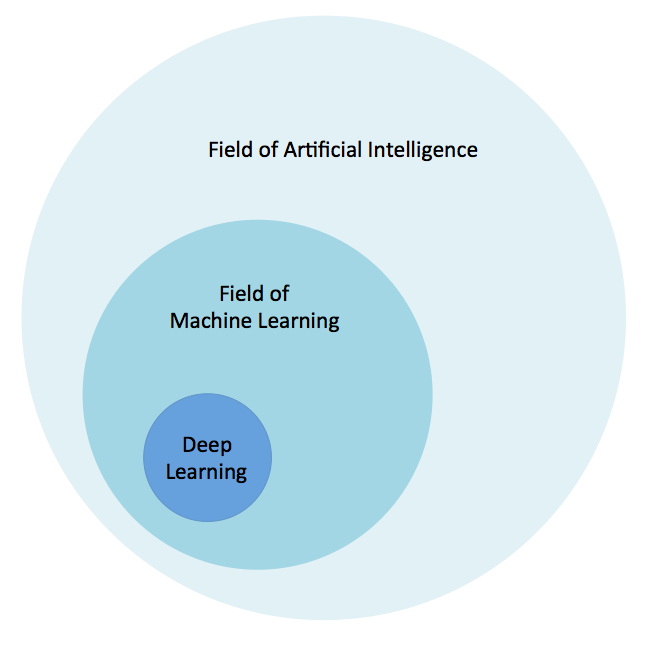
\includegraphics[width=8cm]{figs/ai-ml-dl-relationship.png}
	\caption{Relación entre Inteligencia Artificial, Machine Learning y Deep Learning}
	\label{fig:ai-ml-dl}
\end{figure}

El \textit{Deep Learning} se diferencia del \textit{Machine Learning} convencional, en que están formados por modelos con distintas ramas de procesamiento que son capaces de extraer las representaciones de los datos con varios niveles de abstracción \cite{lecun2015deep}. Mucha de la teoría relacionada se puede encontrar en los años 50 y 60, sin embargo, las aplicaciones y la capacidad de cómputo eran limitadas en la época, hasta ahora donde la capacidad de computación ha crecido a gran escala y en conjunto con las nuevas técnicas propuestas, una mayor cantidad de datos y la aplicación de transformaciones no lineales hacen que esta vertiente viva su época dorada.

Una de las implementaciones más representativas del \textit{Deep Learning} se trata de las redes neuronales, las cuales se encuentran basadas en el funcionamiento del cerebro humano, utilizando el concepto de neuronas que pueden realizar cálculos, la conexión entre las mismas, la función de realizar una tarea específica, etc. Añadir, que se encuentra basado y que el cerebro humano es un sistema mucho más complejo que las redes neuronales y tiene muchos más comportamientos \cite{haykin1994neural}.


Dentro del \textit{Machine Learning}, los algoritmos pueden dividirse según como se realice el entrenamiento del modelo, afectando también a la evaluación y las aplicaciones del mismo. Estas categorias son: \textit{Aprendizaje Supervisado (Supervised Learning), Aprendizaje No Supervidado (Unsupervised Learning) y Aprendizaje Semi-Supervisado (Semi-Supervised Learning)}

\subsection{Aprendizaje Supervisado}

El aprendizaje supervisado se caracteriza por utilizar un conjunto de variables de entrada y encontrar la función que más se aproxime a los valores de salida \cite{Liu2012}. Actualmente es una de las metodologías más utilizadas en \textit{Machine Learning} y es una de las más avanzadas en el campo, sin embargo, la necesidad de los valores de salida (variable dependiente o \textit{target}) requiere que el conjunto de datos se encuentre etiquetado, es decir, para las observaciones de las variables de entrada debe existir la variable de salida para poder general el modelo. En muchos casos este etiquetado se debe de realizar manualmente, por lo que es un proceso que requiere mucho tiempo.

Por otro lado, cabe mencionar que el uso de métodos de aprendizaje supervisado tienen una mayor efectividad que el semi y no supervisado, sin embargo, la necesidad de tener las etiquetas y el coste que ello supone para grandes cantidades de datos, como es en el caso de la detección de anomalías, provocan que se busquen otras soluciones con aprendizajes semi y no supervisado. Además, suele suceder que en la detección de anomalías, éstas sean la menor parte de todos los datos, en otras palabras, la mayor parte de los datos son normales y solo una pequeña porción se trata de anomalías como tal, provocando que el conjunto de datos esté poco compensado.

Uno de los modelos más sencillos de aprendizaje supervisado es la regresión lineal (simple), ésta permite ajustar a una serie de puntos conocidos , \textit{x}, y su respuesta \textit{y} \cite{james2013introduction}, generando una función que permite predecir los valores de \textit{y} con valores no conocidos de \textit{x}:

\begin{equation}
y = ax + b 
\end{equation}

En este caso se predicen los nuevos valores utilizando la función ajustada, existen distintos métodos para encontrar la recta que ajusta los puntos, siendo uno de los más utilizados el ajuste por mínimos cuadrados:

\begin{equation}
a = \frac{\sum(x_i – \bar{x}) (y_i – \bar{y})} {\sum(x_i – \bar{x})^2}
\end{equation}

\begin{equation}
b = y – a \bar{x}
\end{equation}

\begin{figure}[H]
	\centering
	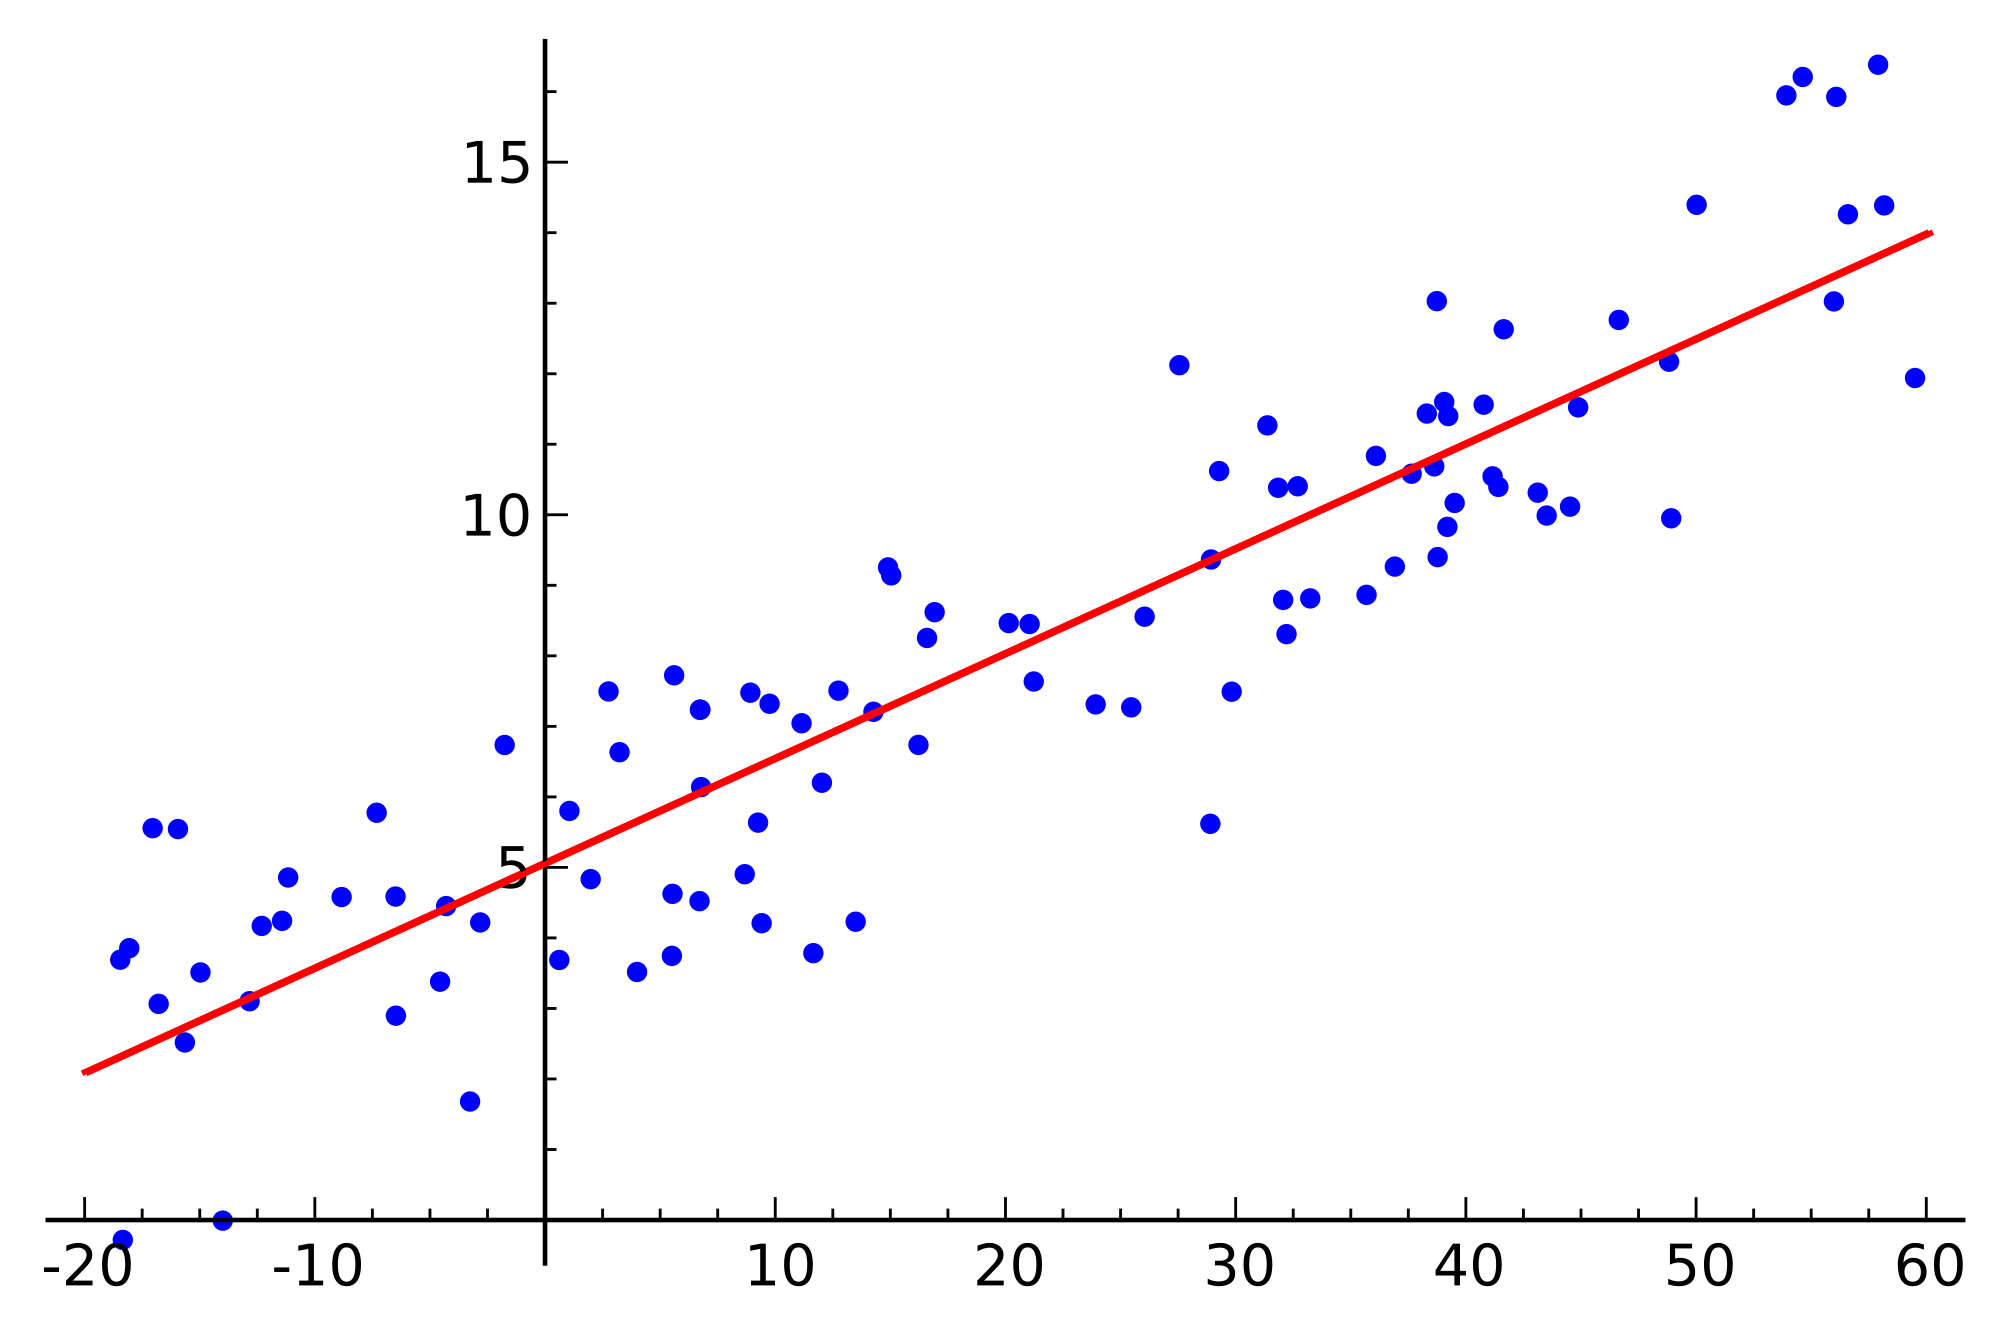
\includegraphics[width=8cm]{figs/Linear_regression.png}
	\caption{Regresión Lineal}
	\label{fig:reglin}
\end{figure}

Como se puede observar en la imagen \ref{fig:reglin}, se ha generado una recta capaz de ajustarse a los puntos y predecir el valor para nuevos puntos. Para generar la función de la recta se ha necesita utilizar la variable dependiente \textit{y} en el entrenamiento para poder generar la función que aproximará los nuevos puntos. 

Durante los siguientes apartados se van a mostrar los distintos modelos utilizados en aprendizaje supervisado para la detección de anomalías, como las redes neuronales artificiales (\textit{Artificial Neural Networks, ANN}, \textit{Gradient Boosting Machines} y \textit{Support Vector Machines}

\subsubsection{Feedforwark Neural Network}

Tal y como se ha comentado anteriormente, las redes neuronales intentan imitar el concepto de la conexión de neuronas del cerebro humano, éstas están formadas por una capa de entrada de datos (\textit{Input}), una capa de salida (\textit{Input}) y un conjunto de capas intermedias, también llamadas capas ocultas (\textit{Hidden}) \cite{haykin1994neural}. En las capas intermedias se encuentran las neuronas conectadas entre sí y pueden estar formadas desde una sola capa, hasta \textit{n} capas, sin embargo, cuanto mayor sea el número de capas, mayor coste de computación asociado. En la siguiente imagen \ref{fig:ANN} podemos ver como sería una arquitectura de una red neuronal:

\begin{figure}[H]
	\centering
	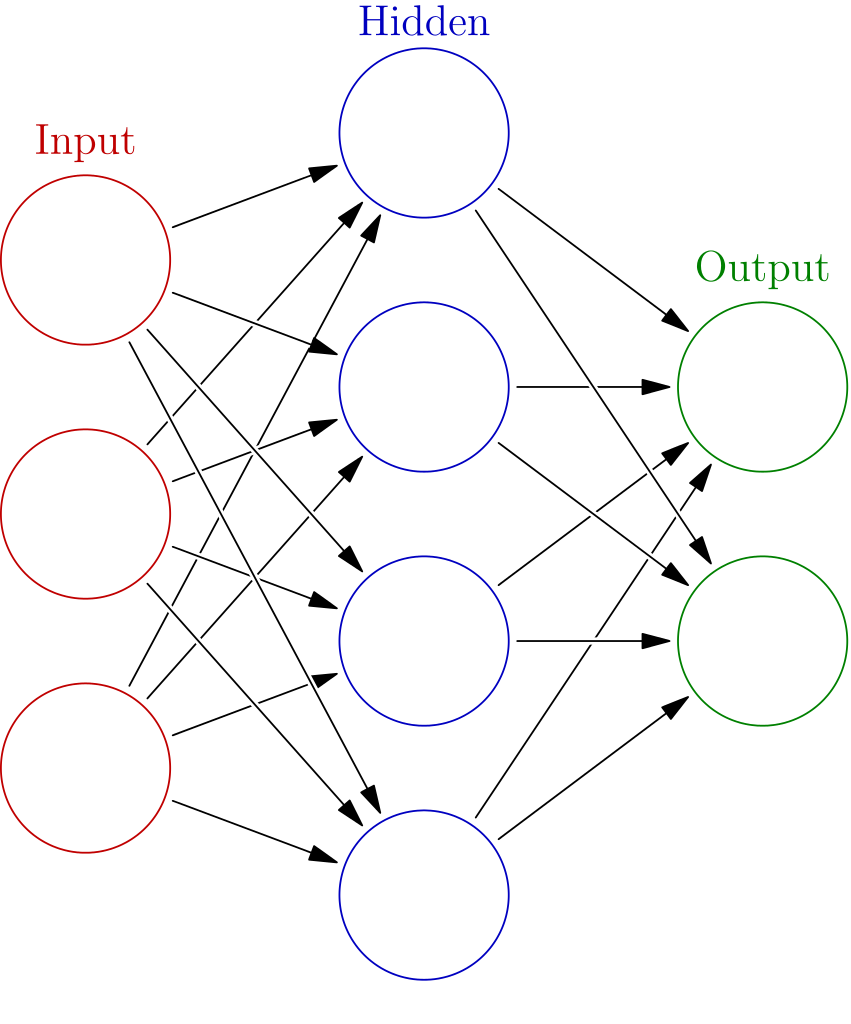
\includegraphics[width=8cm]{figs/Colored_neural_network.png}
	\caption{Red Neuronal Artificial}
	\label{fig:ANN}
\end{figure}

Dentro de las redes neuronales existe un caso base conocido como perceptron, un clasificador binario formado por la capa de entrada, una capa oculta de una sola neurona y una salida \cite{rosenblatt1958perceptron}. El perceptrón ayudará a incluir el concepto de los pesos (\textit{weights}) y el \textit{bias}. 

\begin{figure}[H]
	\centering
	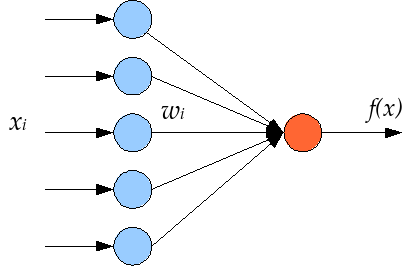
\includegraphics[width=8cm]{figs/Single_layer_perceptron.png}
	\caption{Arquitectura de un Perceptron}
	\label{fig:perceptron}
\end{figure}

Los valores de entrada \(X\) son multiplicados por una serie de pesos \(W\), en una primera instancia se inician aleatoriamente, y se realiza la suma de esta multiplicación, tras la cual se pasará a una función de activación. La función de activación define el valor de salida de la neurona y que se utilizará como valor de entrada para la siguiente neurona o como es en este caso como el valor de salida final. Un ejemplo de una función de activación es la función escalón, donde los valores menores de cero son iguales a cero y los mayores de cero son igual a uno. El \textit{bias} se trata de un pequeño valor que modifica el output sin interactura con las neuronas. De este modo la clasificación de 0 o 1 en un perceptron sería así:

\begin{equation}
    f(x) = g(\sum XW + b)
\end{equation}

Donde \(g(x)\) es la función de activación, X el vector de datos de entrada, W el vector de pesos y b el vector de bias.

\begin{figure}[H]
	\centering
	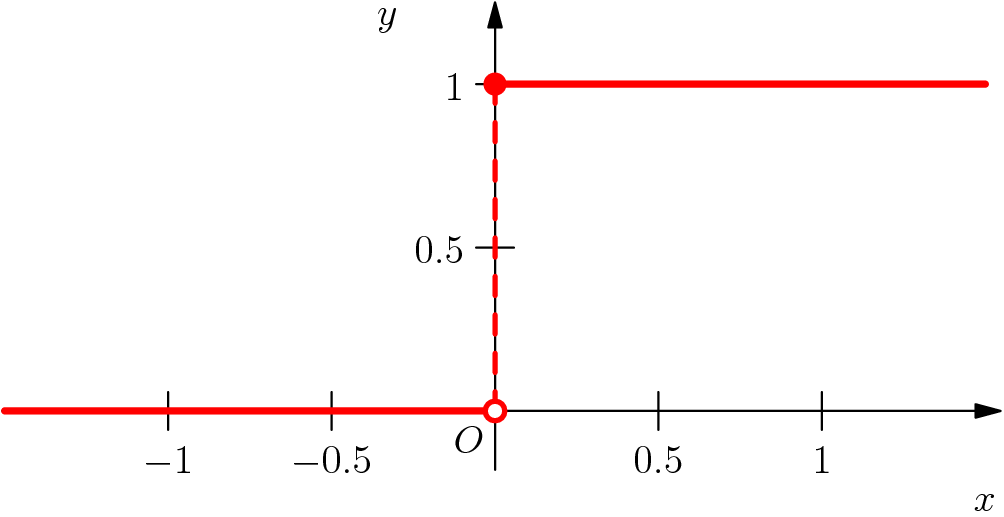
\includegraphics[width=8cm]{figs/stepfunction.png}
	\caption{Función de activación: Función Escalón}
	\label{fig:stepfunction}
\end{figure}

Aumentando la complejidad de la arquitectura, es decir, el número de neuronas, el numero de capas y distintas funciones de activación, se consiguen modelos más complejos pero mantienen el enfoque que se realiza en el perceptron.

Para optimizar la salida, se utilizan varias técnicas de optimización que permiten actualizar los pesos \(W\) y disminuir el error \(E = f(x) - y\), una de las más utilizadas es el \textit{backpropagation}, basado en el descenso del gradiente cuyo objetivo es obtener el gradiente de la función (vector de mayor pendiente) pero utilizar el valor opuesto del mismo multiplicado por un coeficiente de aprendizaje (\textit{learning rate}), una anlogía muy utilizada es imaginar como encontrar el punto más bajo del valle, para ello lo mejor es fijarse en que lugar del punto en el que nos encontremos tiene más pendiente negativa y seguir ese camino. El backpropagation utiliza esté método, pero en lugar de calcular el gradiente sobre la función total (gran coste) se realiza el cálculo de los gradientes locales, empezando desde el punto final de la función.

\begin{figure}[H]
    \centering
    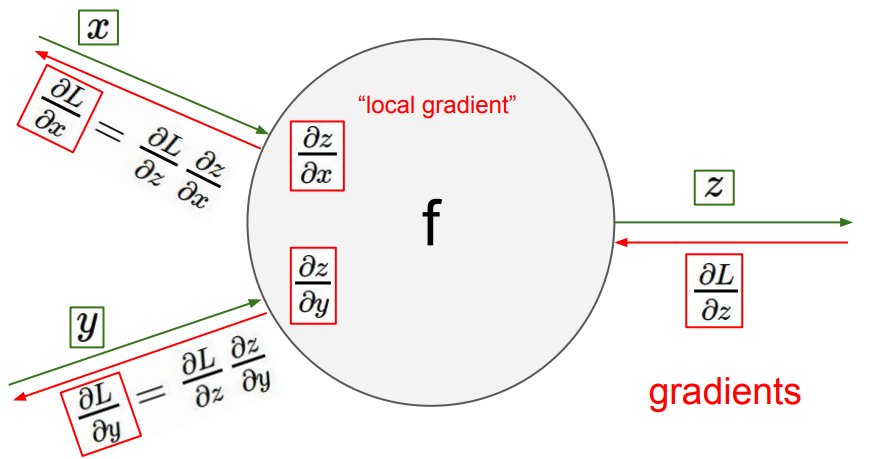
\includegraphics[width=8cm]{figs/backprop.png}
    \caption{Backpropagation}
    \label{fig:backprop}
\end{figure}

La fórmula de la actualización de los pesos en una ANN sería similar a la siguiente:
\begin{equation}
    W_i+1 = W_i - \gamma \frac{1}{n} \sum \nabla L(x,w)
\end{equation}

Donde \(\gamma\) es el \textit{learning rate} y \(L(x)\) es la función de pérdida.

La última capa, la capa de \textit{outputs}, define el número de neuronas de salida, que puede ser igual al número de clases etiquetadas o una sola neurona en el caso de que existan solo dos clases, clasificación binaria. El valor de las salidas irá definido por la función de activación de la última capa de la capa oculta.

\subsubsection{Gradient Boosting Machines}

Las \textit{Gradient Boosting Machines} son uno de los métodos más utilizados actualmente, dada la gran precisión que aportan a la resolución de los problemas. Estos modelos se basan en realizar el ensamblado de modelos débiles, normalmente árboles de decisión, para generar un predictor "fuerte" de una manera iterativa. 

\subsubsection{Support Vector Machines}

\subsection{Aprendizaje No Supervisado}
\subsubsection{Long Short Term Memory Networks}
\subsubsection{Autoencoders}
\subsubsection{Generative Adversarial Networks}
\subsubsection{Recurrent Neural Networks}

\subsection{Aprendizaje Semi-Supervisado}
\subsubsection{Autoencoders}
\subsubsection{Convolutional Neural Networks}
\subsubsection{Generative Adversarial Networks}
\newpage
\chapter{Desarrollo}
\label{chapter:Desarrollo}

En esta parte de la memoria se detallarán los pasos seguidos durante el desarrollo y la aplicación de los algoritmos de \textit{Machine Learning} sobre los datos utilizados. Asimismo, se profundizará en los datos utilizados y cómo se han preprocesado para su posterior aplicación en los algoritmos.

Generalmente, la mayor parte del tiempo de un proyecto de \textit{Data Science} se invierte en la extracción y preprocesado de los datos, hasta que tengan la suficiente calidad como para arrojar resultados fiables tras aplicar los algoritmos. Este ha sido el caso del presente proyecto, la mayor parte de los esfuerzos han recaído en la comprensión de los datos y en cómo hacer frente (tanto por tiempo como por tamaño) a los datos disponibles.

Tanto el preprocesado como la aplicación de los algoritmos de \textit{Machine Learning} se han realizado utilizando el lenguaje de programación \textit{Python} en su versión 3.6 y la exploración y análisis de los datos se han realizado en \textit{Jupyter Notebooks} para facilitar la visualización de los datos y las acciones tomadas. Todo estos procesos se han realizado en una máquina remota proporcionada por la UOC con 10 núcleos y 64gb de memoria RAM.
\newpage

\section{Datos utilizados}

Para este proyecto se va a utilizar un \textit{dataset} con información de las conexiones entre dispositivos IoT, mediante el análisis de los paquetes obtenidos por un analizador de paquetes o \textit{sniffer}, un software que permite observar y recopilar las acciones que desarrollan dentro de una red \cite{sniffer}. Utilizando los datos recopilados por este software se preprocesarán de modo que se pueda extraer la información y posteriormente transformarla y crear nuevas variables.

Los datos iniciales fueron preprocesados inicialmente con la información de las anomalías (únicamente anomalías) que se habían recopilado en un espacio de tiempo de dos meses. En este caso los datos solo contaban con tráfico ilegítimo, por lo que no se podía hacer una detección de anomalías como tal.

Posteriormente, se proporcionaron los datos en bruto en un fichero de extensión \textit{pcap} resultante del \textit{sniffer} mencionado anteriormente. Este fichero contiene información de las distintas capas en las que se almacenan los datos, siendo las de más interés las capas \textit{TCP} e \textit{IP}.

\begin{itemize}
    \item \textit{Transmission Control Protocol}: originario de los años 70/80, consiste en un protocolo para la transmisión de paquetes en conexiones \textit{host} a \textit{host} en redes \cite{postel1981transmission}.
    \item \textit{Internet Protocol}: protocolo que permite la transmisión de datos de origen a destino donde el origen y el destino son direcciones de longitud fija y proporciona los medios para la división y reagrupación de grandes datos en grupos más pequeños \cite{postel1981internet} .
\end{itemize}

Sobre estas capas se obtiene la información disponible al más bajo nivel y posteriormente se generarán nuevas variables en base a los datos obtenidos. Siendo los datos de la capa TCP los siguientes:

\begin{itemize}
    \item Puerto de origen: indica el puerto de origen utilizado para realizar la conexión desde la IP de origen.
    \item Puerto de destino: indica el puerto de destino utilizado en la conexión entre \textit{hosts}.
\end{itemize}
\newpage

Los datos obtenidos de la capa IP:
\begin{itemize}
    \item IP de origen: dirección con longitud fija del origen de la conexión.
    \item IP de destino: dirección con longitud fija del destino de la conexión.
    \item \textit{Length}: longitud/tamaño de los paquetes enviados durante la conexión.
\end{itemize}

\begin{figure}[H]
    \centering
    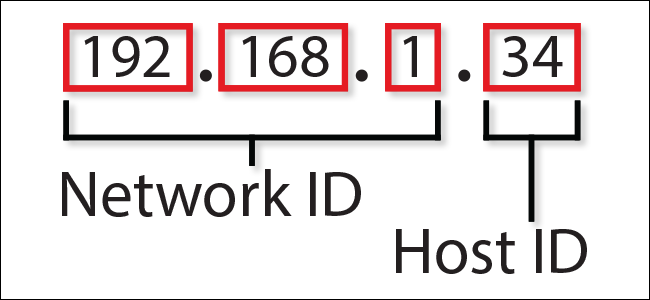
\includegraphics[width=6cm]{figs/ip.png}
    \caption{Ejemplo de dirección IPv4}
    \label{fig:wireshark}
\end{figure}

Otros datos:

\begin{itemize}
    \item \textit{Payload}: contenido de los datos transmitidos, pudiendo ser texto, imágenes o comandos a ejecutar en el \textit{host} de destino, con posibilidad de estar cifrado.
    \item \textit{Timestamp}: marca de tiempo que indica en qué momento se realizó la conexión.
\end{itemize}

Un ejemplo más visual de los datos a bajo nivel se puede realizar utilizando la herramienta \textit{Open Source, Wireshark}, fundamental a la hora de entender cómo están distribuidos los datos en las capas.

\begin{figure}[H]
    \centering
    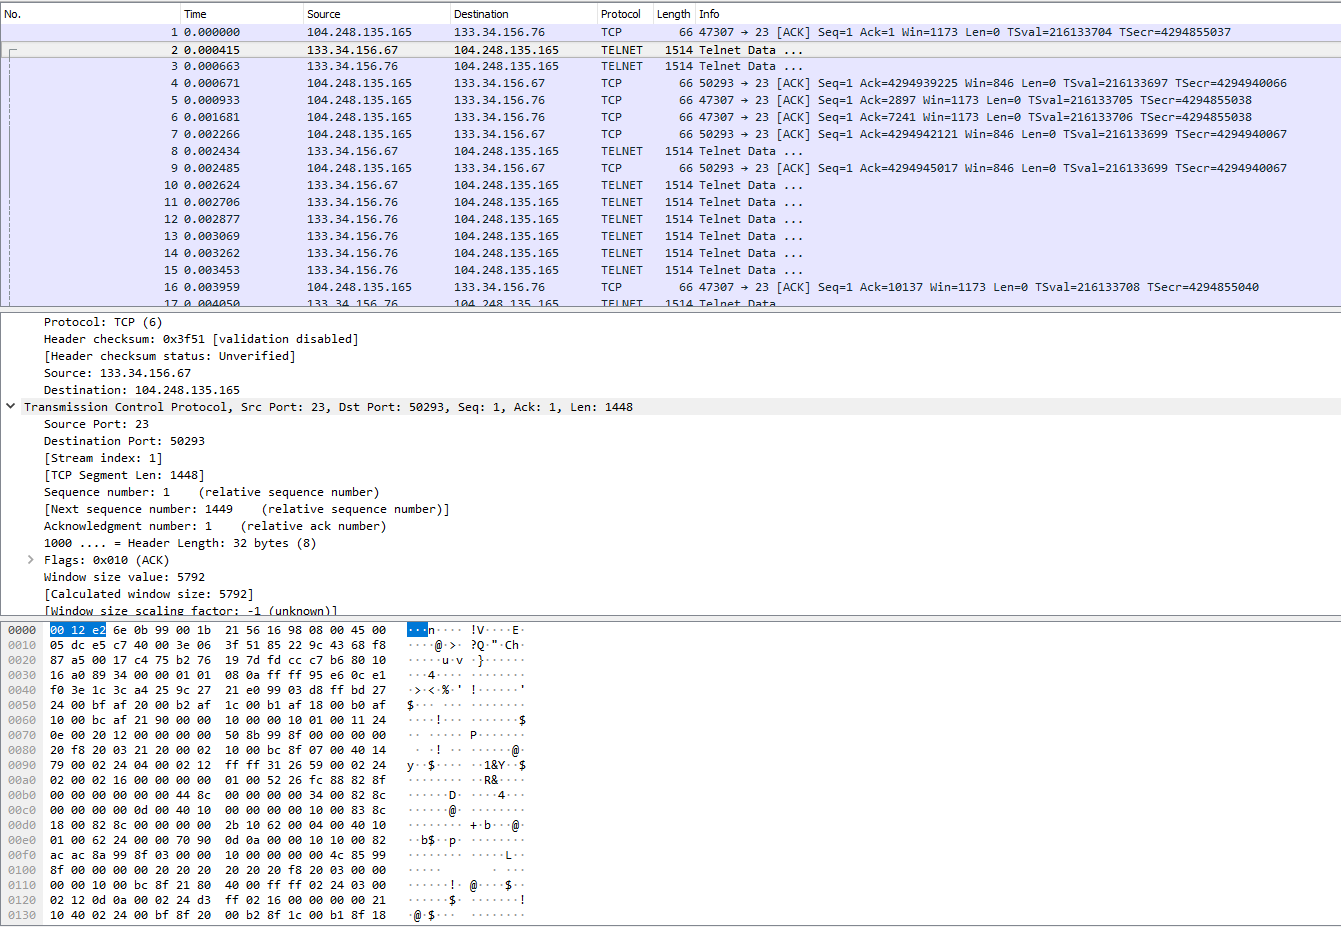
\includegraphics[width=15cm]{figs/wireshark.PNG}
    \caption{Ejemplo de datos pcap en Wireshark}
    \label{fig:wireshark}
\end{figure}

El \textit{Timestamp} puede indicar que el problema debería tratarse como una serie temporal y generar variables en base a esta característica.

Los datos provienen de la recolección de información realizada el 2 de Febrero de 2019, contando tanto con tráfico legítimo como ilegítimo. Sin embargo, no existe clasificación de los datos, por lo que se trata de un problema de carácter no supervisado y como consecuencia se utilizarán técnicas como las descritas en el capítulo \ref{chapter:Estado del Arte} de aprendizaje no supervisado.

\newpage

\section{Exploración y Preprocesamiento}

En este aportado se van a mostrar los pasos seguidos durante la exploración y  el procesamiento asicomo la información obtenida durante el proceso. Ambas etapas se realizan de manera conjunta, es decir, la exploración conlleva la realización de distintos preprocesamientos o otras palabras, se realiza \textit{Feature Engineering}. Se puede definir como el proceso de exploración y procesamiento de datos que ayudan a la creación de nuevas variables que puedan mejorar la eficiencia del modelo\cite{fe}.

El paso inicial era la extracción de los datos del fichero \textit{pcap}, el tamaño total era cercano a los 14 GB, de modo que en el momento de cargar la información en memoria, el uso aumentaba considerablemente dificultando su manipulación, por lo que el primer paso fue investigar si existía alguna forma de dividirlo. El resultado fue el uso de la herramienta \textit{tcpdump}, una línea de comandos utilizada para el análisis de paquetes escrita en C/C++ \cite{tcpdump}, la misma permitía la división del fichero original en pequeños ficheros con el tamaño deseado. La división se realizó con un tamaño máximo de 500 MB, para permitir la posterior paralelización de los ficheros y evitar un uso muy alto de memoria, dando como resultado 15 ficheros.

Una vez obtenidos los ficheros se deben procesar de modo que el resultado sean datos de forma tabular, que puedan ser explorados y preprocesados con mayor facilidad. Para realizar este proceso se utilizó el módulo de \textit{python}, \textit{scapy}, utilizado comúnmente en tareas de análisis de redes. Gracias a la granularidad de los nuevos ficheros y a utilizar \textit{python} se procesan 9 ficheros simultáneamente utilizando el módulo mencionado, éste se encarga de recorrer las capas mencionadas y extraer los datos y organizarlos de forma tabular, concretamente en \textit{csv}. En ciertos casos, los paquetes pueden contener el \textit{payload}, cuando este es el caso se extrae y se añade como una columna más, para el resto se trata como si fueran \textit{NA} o datos sin registro. 

Una vez terminado el proceso se obtienen los primeros datos en brutos de carácter estructurado. Se genera una cantidad análoga de ficheros con un volumen tres veces superior a los datos originales, con las variables mencionadas en la sección anterior. Antes de realizar ningún tipo de exploración se realiza un preprocesado en paralelo para generar nuevas variables sencillas que puedan aportar información de cara a la primera exploración. Las nuevas variables son las siguientes:

\begin{itemize}
    \item Red 1 IP origen
    \item Red 2 IP origen
    \item Red 3 IP origen
    \item Host IP origen
    \item Red 1 IP destino
    \item Red 2 IP destino
    \item Red 3 IP destino
    \item Host IP destino
    \item is\_busybox
    \item is\_sh
    \item is\_enable
\end{itemize}

Las variables en referencia a las IPs se generaron haciendo una división de las direcciones:

\begin{equation}
    192.168.1.1 => 192_{red1}\; 168_{red2}\; 1_{red3}\; 1_{host}
\end{equation}

El resto de las variables se obtuvieron mediante el \textit{parseo} del \textit{payload} en aquellos registros que así lo tuvieran y buscando la existencia de las palabras clave \textit{sh, enable y busybox}, siendo la mayor parte de los registros sin contenido en el \textit{payload} o incluso cifrado. La razón por la que se eligieron estas palabras clave es por el uso de este tipo de comandos en los dispositivos IoT por \textit{malwares} conocidos, \textit{busybox} se trata de una versión mínima de un sistema operativo \textit{UNIX} utilizado en pequeños dispositivos y que puede ser explotado por \textit{malware}\cite{ibmiot}.  De la misma manera \textit{sh} y \textit{enable} son comandos comúnmente utilizados en este tipo de ataques. Las tres variables son de tipo binario, es decir, indica si en el registro existe el comando o no.

El proceso de exploración se realiza en \textit{Jupyter Notebooks} con la ayuda del módulo \textit{matplotlib} y \textit{seaborn} para las visualizaciones. Para esta primera exploración, se van a buscar los medios más utilizados en las distintas conexiones, es decir, las IPs más utilizadas, puertos más utilizados, información de las variables binarias y la evolución de la cantidad de conexiones en el tiempo.

\begin{figure}[H]
    \centering
    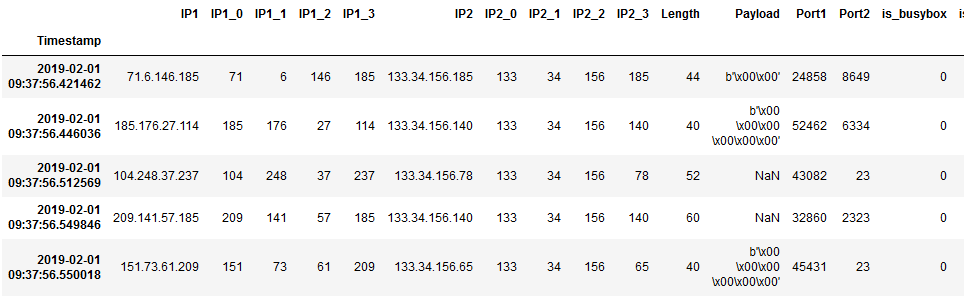
\includegraphics[width=15cm]{figs/initial_data.PNG}
    \caption{Datos en forma tabular}
    \label{fig:tabulardata}
\end{figure}

Para realizar la exploración se unen todos los datos contenidos en los ficheros generados ordenados por la marca de tiempo. Una vez cargados, se realizan las operaciones básicas para determinar que no faltan datos, es decir, que en las variables originales (salvo el \textit{payload}) no falta ningún tipo de registro. En este caso no hay existencia de \textit{NAs} en las variables, en otras palabras, todos los datos tienen los registros necesarios.

En la siguiente gráfica se puede observar la cantidad de valores únicos en cada variable, en la que se pueden apreciar dos cosas claras:

\begin{itemize}
    \item Las variables con más únicos son las de los puertos.
    \item No hay una gran cantidad de IPs únicas.
\end{itemize}

\begin{figure}[H]
    \centering
    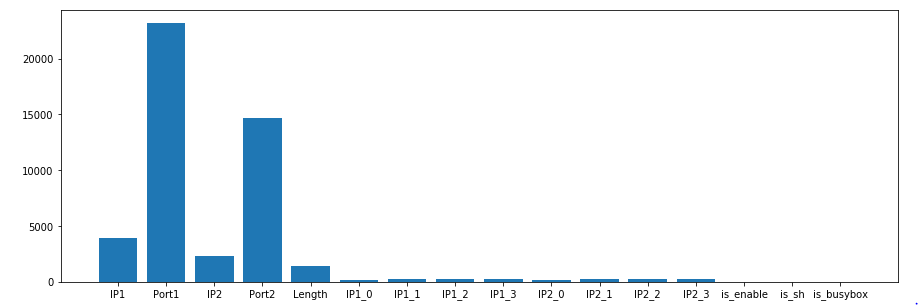
\includegraphics[width=17cm]{figs/unique_vals.PNG}
    \caption{Cantidad de valores únicos en las variables}
    \label{fig:uniquevals}
\end{figure}

La parte de los puertos en origen (subíndice 1) tiene sentido que sea mayor que en la IP destino, dado que a la hora de iniciar conexiones por lo general el puerto origen es aleatorio y el de destino suele ser fijo, como el puerto 22 para conexiones \textit{ssh}, por lo que puede significar que se estuviera haciendo un escaneo de puertos. Esto se puede ver en el diagrama de barras representando los puertos más utilizados en origen y destino:


\begin{figure}[H]
    \centering
    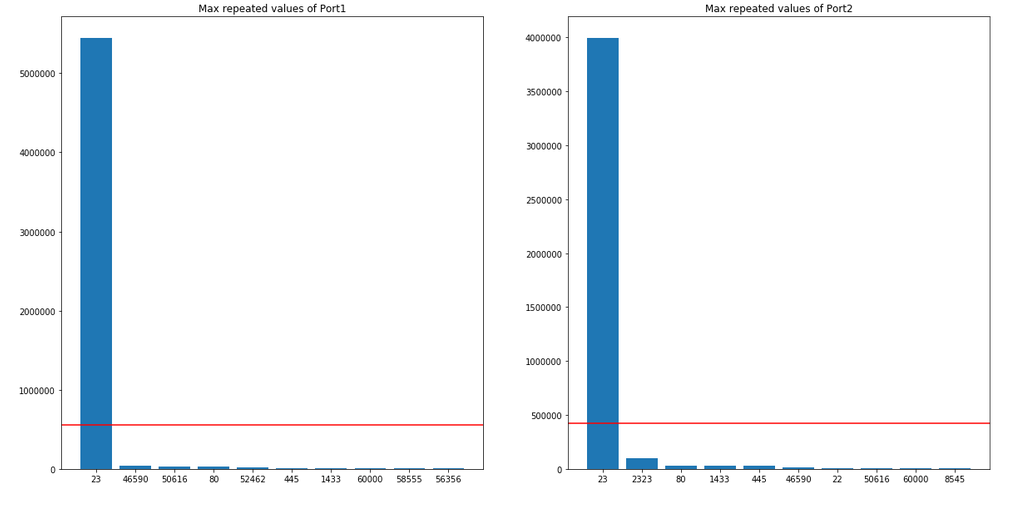
\includegraphics[width=17cm]{figs/ports.PNG}
    \caption{Puertos más utilizados}
    \label{fig:ports}
\end{figure}

Se puede observar lo siguiente:

\begin{itemize}
    \item EL puerto más utilizado en ambos casos con diferencia es el puerto 23. Es el puerto utilizado para realizar las conexiones vía \textit{telnet}.
    \item Seis de los diez puertos más utilizados en la IP de origen son puertos aleatorios, utilizados al realizar la conexión. Los puertos del rango 4xxxx-6xxxx caen en este uso efímero.
    \item El puerto 80 por lo general es utilizado en conexiones \textit{HTTP} (web).
    \item El puerto 445 es utilizado para la transferencia de ficheros.
    \item El puerto 1433 suele utilizarse en conexiones de \textit{Microsoft SQL Server}.
    \item El 2323 puede ser un puerto alternativo para la conexión vía \textit{telnet}\cite{telnetport}.
    \item El puerto 22 se utiliza para conexiones \textit{ssh}.
    \item Tanto para destino como para origen se repiten los puertos 46590, 50616 y 60000, cayendo en el rango de puertos temporales.
\end{itemize}

En el caso de las IPs más utilizadas se puede ver lo siguiente:

\begin{figure}[H]
   \begin{minipage}{0.48\textwidth}
     \centering
     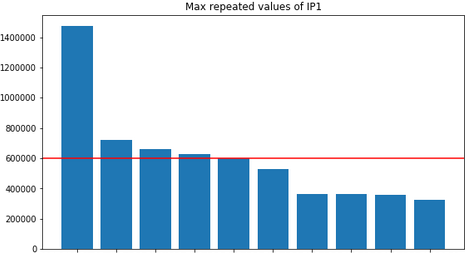
\includegraphics[width=1\linewidth]{figs/ip1.PNG}
     \caption{IPs de origen con la mayor cantidad de conexiones}
     \label{Fig:ip1}
   \end{minipage}\hfill
   \begin{minipage}{0.48\textwidth}
     \centering
     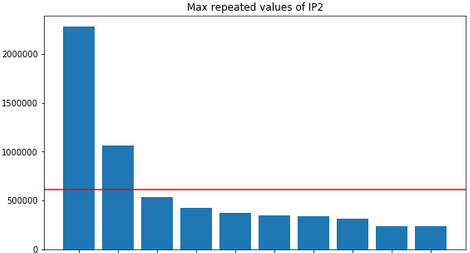
\includegraphics[width=1\linewidth]{figs/ip2}
     \caption{IPs de destino con la mayor cantidad de conexiones}
     \label{Fig:ip2}
   \end{minipage}
\end{figure}

Con una cantidad de datos cercana a los 11 millones de registros la mayor parte de las conexiones se registran en estos diez valores máximos con una diferencia de casi el doble de la primera a la segunda tanto para origen como destino.

Dentro de la temporalidad de las conexiones se pueden observar patrones de las conexiones a lo largo del día y su evolución. Debido a la granularidad de los tiempos (capturan con un detalle de microsegundos) estos patrones se han agrupado en distintas ventanas, de modo que en ventanas más pequeñas se puedan detectar ascensos y descensos bruscos, mientras que en las ventanas grandes se puede observar el patrón general. Por ello se han realizado gráficas con ventanas de 1 minuto, 5 minutos y 30 minutos.

\begin{figure}[H]
    \centering
    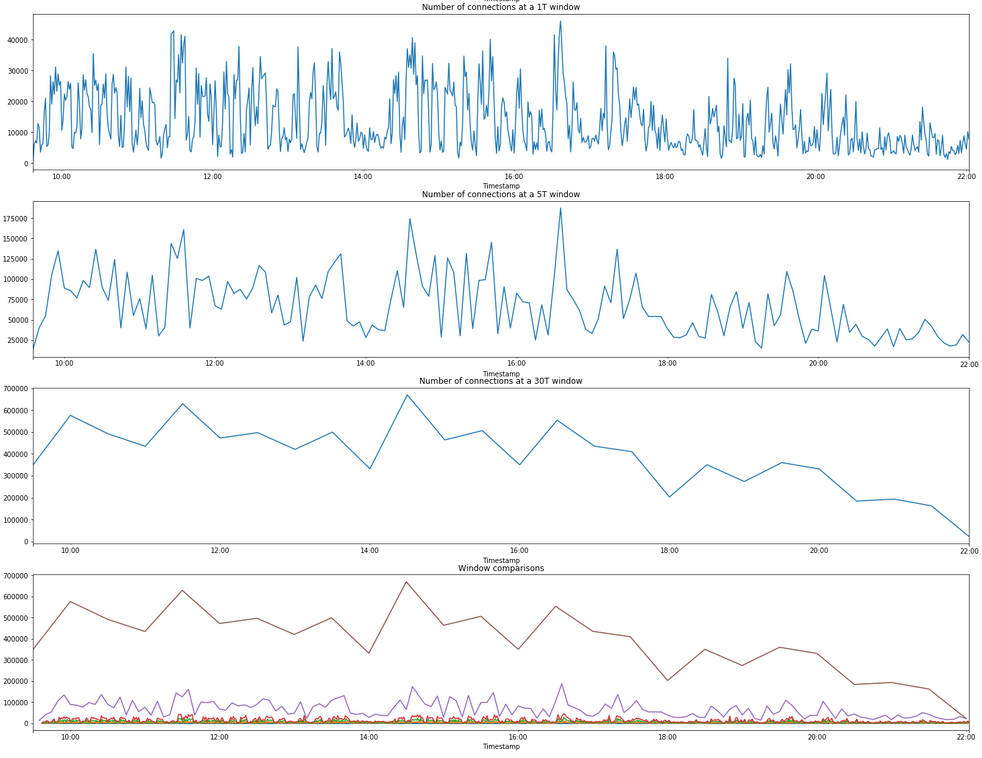
\includegraphics[width=17.5cm]{figs/daily_connections.PNG}
    \caption{Evolución de las conexiones a lo largo del tiempo con distintas ventanas}
    \label{fig:dailyconn}
\end{figure}

Se observa:

\begin{itemize}
    \item Un patrón claro de la cantidad de conexiones, comienza a aumentar durante la mañana y la cantidad de peticiones disminuye por la tarde
    \item En ventanas más pequeñas existe una caída cerca de las 11 horas y un pequeño pico después.
    \item Se aprecia un pequeño valle a las 14:00, más pronunciado en ventanas pequeñas.
    \item Gran caída sobre las 18:00.
    \item En las comparaciones entre ventanas, se aprecia como el patrón es semejante entre ellas.
\end{itemize}

En cuanto a las variables binarias, se observa que se encuentran muy descompensadas y existen pocas observaciones que las contengan:

\begin{table}[H]
    \centering
    \begin{tabular}{|c|c|c|c|}
    \hline
    \; & is\_busybox & is\_enable & is\_sh \\ [0.5ex]
    \hline
        \textbf{0} & 9812548 & 10114993 & 9643741 \\
        \textbf{1} & 358980 & 56535 & 527787 \\ [1ex]
    \hline
    \end{tabular}
    \caption{Tabla de frecuencias de las variables binarias}
    \label{tab:bintable}
\end{table}

Por último, en la exploración inicial se observo la distribución de la variable \textit{Length}. En la figura \ref{fig:lenhist} se puede apreciar como la mayor parte de las conexiones se realizan con una longitud muy pequeña,  recayendo la mayor parte de los valores en torno a 40-50 o con una magnitud grande, generalmente en torno a los 1400, mientras que los valores intermedios son minoría.

\begin{figure}[H]
    \centering
    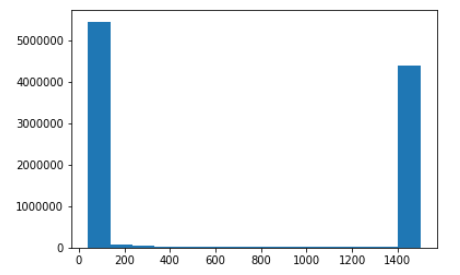
\includegraphics[width=10cm]{figs/lenhist.PNG}
    \caption{Histograma de la variable \textit{Length}}
    \label{fig:lenhist}
\end{figure}

Sobre la variable \textit{Payload} no se realizó ningún tipo de exploración, a parte del parseo, debido a la dificultad de procesar los datos y adaptarlos a un formato más tabular. Se trató de obtener la secuencia de comandos en aquellas observaciones no cifradas sin embargo, no se consiguió obtener esta secuencia que podría haber ayudado en gran medida aportando una gran cantidad de información. Algnas de las variables que se podrían haber obtenido son: cantidad de comandos en secuencia, longitud media de los comandos o incluso técnicas de NLP como \textit{Tf-idf (Term frequency – Inverse document frequency)}.

Con la información obtenida y con un mayor conocimiento de los datos disponibles, se propusieron nuevas variables que podrían aportar más información y podrían ser más útiles a los modelos (en este momento aún por decidir). Tras varios intentos se generaron las siguientes variables:

\begin{itemize}
    \item \textit{IP1\_time\_diff\_per\_value}: tiempo en segundos, de la diferencia de tiempos desde la anterior conexión y la conexión actual de la IP de origen. 
    \item \textit{IP2\_time\_diff\_per\_value}: tiempo en segundos, de la diferencia de tiempos desde la anterior conexión y la conexión actual de la IP de destino.
    \item \textit{IP1\_IP2\_time\_diff\_per\_value}: tiempo en segundos, de la diferencia de tiempos desde la anterior conexión y la conexión actual entre IPs únicas de origen y destino.
    \item \textit{Port1\_last\_1}: cantidad de puertos únicos utilizados por la IP de origen en una ventana de un minuto
    \item \textit{Port2\_last\_1}: cantidad de puertos únicos utilizados por la IP de destino en una ventana de un minuto
\end{itemize}

Todas estas variables se generan en especifico para los valores únicos de las IPs, es decir, cuando se utiliza la IP de origen, se itera entre todos los valores únicos y por cada valor se genera la ventana o la diferencia de tiempo. Con esto se consigue que las nuevas variables solo estén relacionadas con las mismas IPs, tanto de origen, destino o para el caso de \textit{IP1\_IP2\_time\_diff\_per\_value} de ambas y que no dependan de conexiones entre distintas IPs.

Con las nuevas variables se pretende conseguir distintos tipos de información, con la diferencia de tiempo en la IP de origen, se pretende observar si se está utilizando asiduamente, esta teniendo un pico de conexiones o si por el contrario las establece raramente. Por otro lado, para la IP de destino se pretende observar si esta siendo objetivo de muchas conexiones en cortos periodos de tiempo, que podrían significar ataques \textit{DDoS (Distributed Denial of Service)}. Para la diferencia entre las conexiones únicas de IP se pretende obtener si se pueden estar realizando escaneos de puertos sobre la IP de destino. En el caso de las variables de puertos, su finción es obtener información más precisa de si puede estar realizando un escaneo o existen IPs de origen con muchas conexiones simultáneas que observan distintos destinos.

Una vez generadas estas variables, se necesita observar la cercanía (o distancia) entre las redes, puesto que es muy común que una vez se infecte un dispositivo, éste intente infectar aquellos dispositivos que se encuentren en su misma red o una red cercana. Inicialmente se planteo utilizar la IP como variable numérica y obtener la distancia euclídea entre la IP origen y destino, sin embargo, no existe ningún tipo de relación entre ellas de esta manera, es decir, la IP 1 y 2 no están a la misma distancia que las IPs 230 y 231. Aprovechando las variables generadas de las IPs con las subredes y el host, se podría calcular la distancia entre ellas, sin embargo, en este caso tomaría como equivalente la distancia entre hosts y la distancia entre redes principales sin embargo, redes con distinto valor no están relacionadas mientras que si la única diferencia es en el host, estos se encuentran en la misma red.

\begin{equation}
    dist(IP_{red1}, IP_{red2}) \neq  dist(IP_{host1}, IP_{host2})
\end{equation}

Para ello se tomó la IP como un espacio 4-dimensional (red1, red2, red3 y host) con valores ponderados, 1000 para la primera red, 100 para la segunda, 10 para la tercera y uno para el host.

\begin{equation}
    IP_x = (x_1, x_2, x_3, x_4)
\end{equation}
\begin{equation}
    dist(IP_x, IP_y) = \sqrt{1000*(x_1 - y_1)^2 + 100*(x_2 - y_2)^2 + 10*(x_3 - y_3)^2 + (x_4 - y_4)^2}
\end{equation}

Con esto una diferencia de uno en la red principal, daría una distancia de \(\sqrt{1000} \approx 32\).

Tras realizar pruebas con este tipo de distancia, se decidió utilizar otro enfoque mejorando los resultados. En lugar de tomar la IP como un valor 4-dimensional, se tomo como 32-dimensional, es decir, una dimensión por cada bit.

\begin{equation}
    IP = 192.128.1.1 = 11000000100000000000000100000001
\end{equation}

Para dar aún más peso a los valores iniciales y la cercanía a nivel de red se utilizo el operador \textit{XOR}, devolviendo un 1 para cuando existe diferencia entre los bits de la misma posición o 0 si el valor es igual. Una vez aplicado el operador, se cuentan el número de ceros por la izquierda, en otras palabras, el número de bits iniciales (redes principales) que coinciden, al momento que aparece una diferencia se para de contar. El número resultante se le resta a 32 y se divide entre 32 para normalizar el valor entre 1 y 0, siendo el uno redes completamente distintas y el cero la misma red y el mismo host. Podemos ver el siguiente ejemplo entre IPs que solo se diferencia en el host:


\begin{gather*}
IP_1 = 192.128.1.1 = 11000000100000000000000100000001 \\
IP_2 = 192.128.1.2 = 11000000100000000000000100000010 \\
XOR(IP_1, IP_2) = 00000000000000000000000000000010 \\
n_{zeros} = 31 \\
dist(IP_1, IP_2) = \frac{(32 - n_{zeros})}{32} = \frac{1}{32}
\end{gather*}

En el caso de diferencias entre redes:

\begin{gather*}
    IP_3 = 255.128.1.1 = 11111111100000000000000100000010 \\
    XOR(IP_1, IP_3) = 00111111100000000000000000000000 \\
    n_{zeros} = 2 \\
    dist(IP_1, IP_3) = \frac{(32 - n_{zeros})}{32} = \frac{30}{32}
\end{gather*}

Como se puede observar la distancia aumenta en gran medida con las redes y en muy poca con los host, aportando más valor como nueva variable que las distancias utilizadas inicialmente.

Una creadas las nuevas variables se realiza otra exploración con el fin de identificar si pueden ser útiles y si es así como tratarlas de cara a la detección de anomalías. Siendo uno de los primeros pasos la correlación entre las variables visualizándolo todo en un \textit{heatmap}:

\begin{figure}[H]
    \centering
    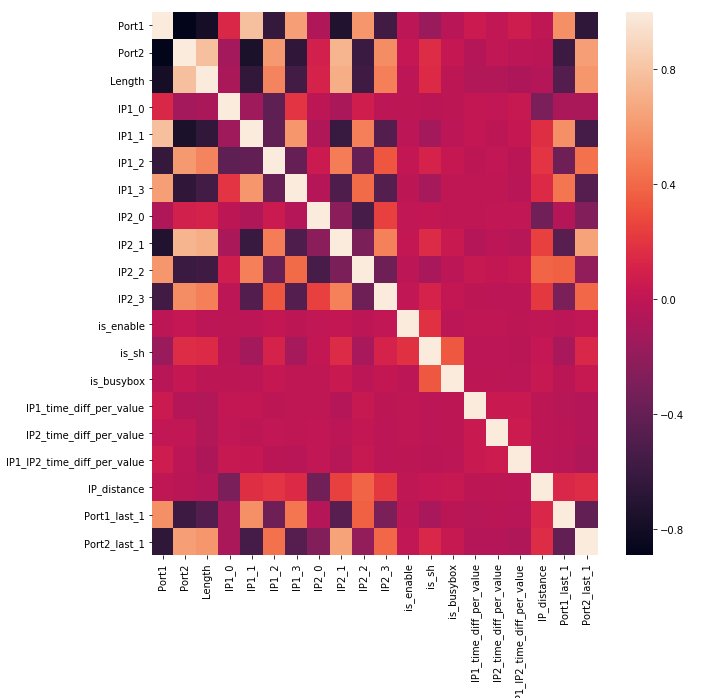
\includegraphics[width=10cm]{figs/corr.PNG}
    \caption{Mapa de correlaciones}
    \label{fig:corr}
\end{figure}

Se pueden observar lo siguiente:

\begin{itemize}
    \item Correlación entre los puertos negativa, posiblemente por la asignación de puertos por encima de 40000 en el inicio de las conexiones.
    \item A mayor número de puerto menor \textit{Length}.
    \item No existen correlaciones entre las redes, subredes y hosts de las IPs.
    \item Parece que a mayor puerto de destino, mayor \textit{Length}.
    \item Las distintas variables de diferencia de tiempo parecen no estar correladas entre sí.
    \item La cantidad de puertos en el último minuto están negativamente correladas entre ellas.
\end{itemize}

Para las diferencias de tiempo se observan que la mayor parte se encuentran en valores muy pequeños, inferiores a un segundo en la IP de origen ,\ref{Fig:ip1_diff1} \ref{Fig:ip1_diff2}. Este comportamiento se repite también para la IP destino, pero ésta contiene más valores dentro del rango inferior a un segundo que la IP de origen \ref{Fig:ip2_diff1} \ref{Fig:ip2_diff2}. En el caso de la diferencia conjunta, el patrón es muy similar a la IP de destino pero con una cantidad menor de observaciones, en otras palabras, hay IPs únicas que solo se han conectado una vez y no tienen diferencia de tiempo \ref{Fig:ip12_diff1} \ref{Fig:ip12_diff2}.

\begin{figure}[H]
   \begin{minipage}{0.48\textwidth}
     \centering
     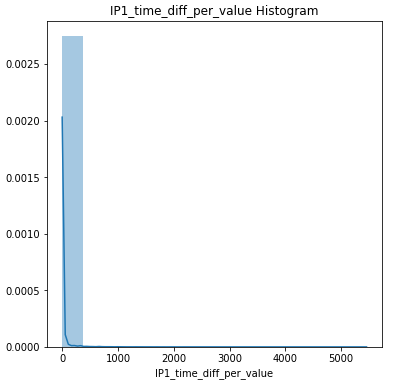
\includegraphics[width=0.8\linewidth]{figs/ip1diff_1.PNG}
     \caption{Distribución total de \textit{IP1\_time\_diff}}
     \label{Fig:ip1_diff1}
   \end{minipage}\hfill
   \begin{minipage}{0.48\textwidth}
     \centering
     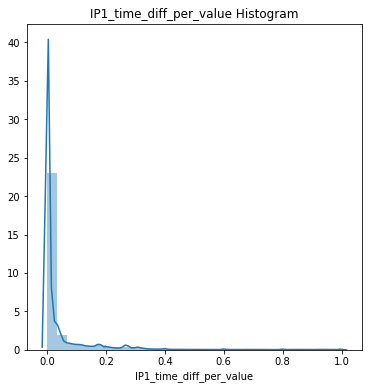
\includegraphics[width=0.8\linewidth]{figs/ip1diff_2.PNG}
     \caption{Distribución para valores menores a un segundo de \textit{IP1\_time\_diff} }
     \label{Fig:ip1_diff2}
   \end{minipage}
\end{figure}

\begin{figure}[H]
   \begin{minipage}{0.48\textwidth}
     \centering
     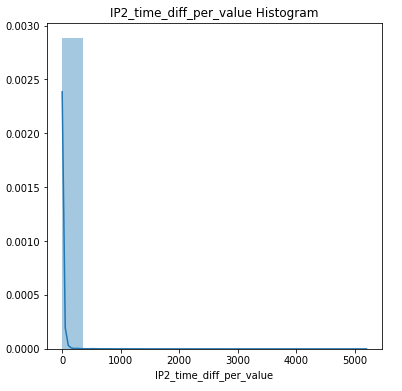
\includegraphics[width=0.8\linewidth]{figs/ip2diff_1.PNG}
     \caption{Distribución total de \textit{IP2\_time\_diff}}
     \label{Fig:ip2_diff1}
   \end{minipage}\hfill
   \begin{minipage}{0.48\textwidth}
     \centering
     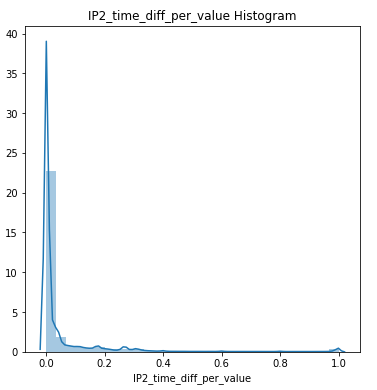
\includegraphics[width=0.8\linewidth]{figs/ip2diff_2.PNG}
     \caption{Distribución para valores menores a un segundo de \textit{IP2\_time\_diff} }
     \label{Fig:ip2_diff2}
   \end{minipage}
\end{figure}

\begin{figure}[H]
   \begin{minipage}{0.48\textwidth}
     \centering
     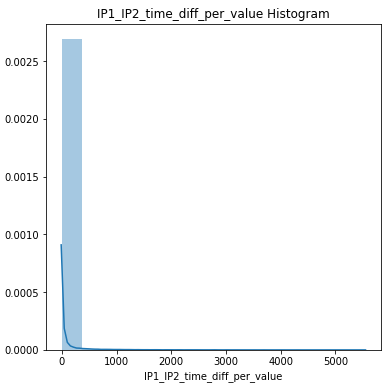
\includegraphics[width=0.8\linewidth]{figs/ip12diff_1.PNG}
     \caption{Distribución total de \textit{IP1\_IP2\_time\_diff}}
     \label{Fig:ip12_diff1}
   \end{minipage}\hfill
   \begin{minipage}{0.48\textwidth}
     \centering
     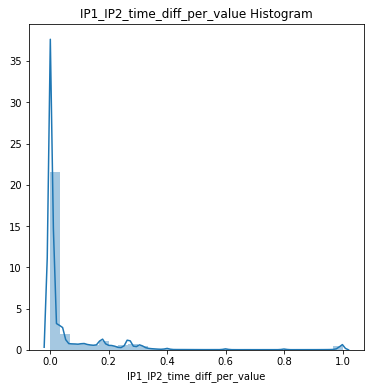
\includegraphics[width=0.8\linewidth]{figs/ip12diff_2.PNG}
     \caption{Distribución para valores menores a un segundo de \textit{IP1\_IP2\_time\_diff} }
     \label{Fig:ip12_diff2}
   \end{minipage}
\end{figure}

\begin{figure}[h]
    \centering
    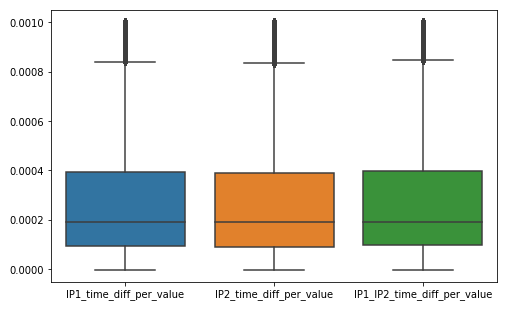
\includegraphics[width=10cm]{figs/ipdiff_comp.PNG}
    \caption{Digrama de cajas según diferencia de tiempo}
    \label{fig:ipdiff_comp}
\end{figure}

Otra variable a tomar en cuenta es la distancia entre IPs. Dentro de la exploración (\ref{fig:ipdist}) se ha observado como la gran mayoría de las IPs provienen de redes completamente distintas, muy pocas IPs comparten la primera red y solo unas pocas observaciones comparten más que los primeros 8 dígitos.

\begin{figure}[H]
    \centering
    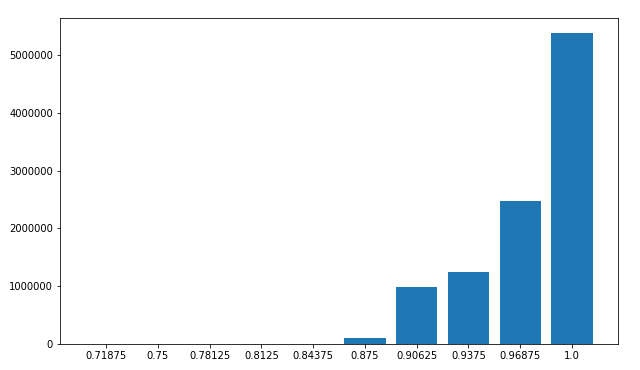
\includegraphics[width=10cm]{figs/ip_distance.PNG}
    \caption{Diagrama de barras de la distancia entre IPs}
    \label{fig:ipdist}
\end{figure}

En cuanto a los puertos y al número de puerto utilizados en el último minuto aparecen cosas interesantes:

\begin{itemize}
    \item La mayor parte de los registros han utilizado de 2 a 7 puertos distintos en el último minuto, tanto para destino como origen.
    \item La distribución muestra que hay una gran cantidad de registros que han utilizado de 30 a 50 puertos en el último minuto.
    \item La cantidad de puertos en el último minuto en origen contiene registros con un gran número de puertos.
\end{itemize}

\begin{figure}[H]
   \begin{minipage}{0.48\textwidth}
     \centering
     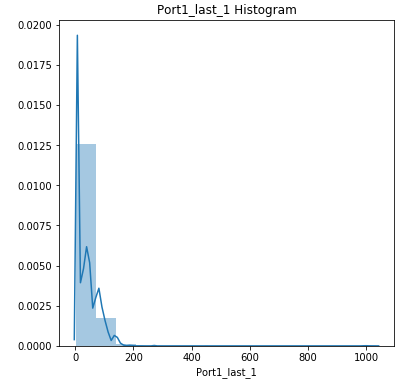
\includegraphics[width=0.8\linewidth]{figs/port1_last.PNG}
     \caption{Distribución de número de puertos en el último minuto de origen}
     \label{Fig:port_time1}
   \end{minipage}\hfill
   \begin{minipage}{0.48\textwidth}
     \centering
     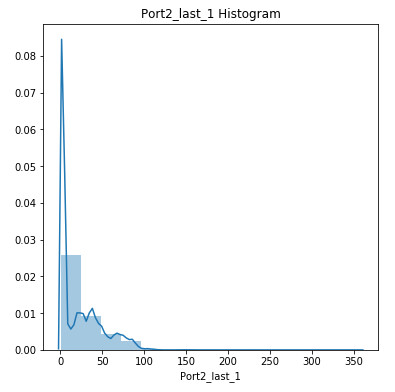
\includegraphics[width=0.8\linewidth]{figs/port2_last.PNG}
     \caption{Distribución de número de puertos en el último minuto de destino}
     \label{Fig:port_time2}
   \end{minipage}
\end{figure}

\begin{itemize}
    \item Los puertos están más distribuidos en destino.
    \item Los puertos en origen están más centrados en valores bajos
    \item Se pueden apreciar patrones de conexión cruzando los puertos
\end{itemize}

\begin{figure}[H]
   \begin{minipage}[b]{0.48\textwidth}
     \centering
     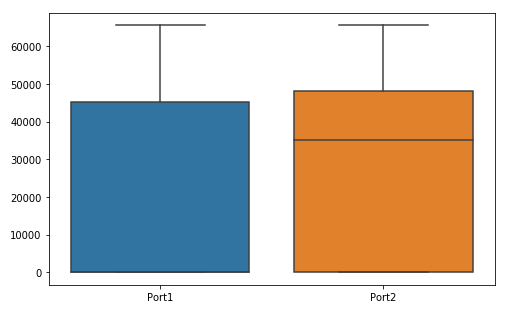
\includegraphics[width=0.8\linewidth]{figs/dist_ports.PNG}
     \caption{Diagramas de caja de los puertos en origen y destino}
     \label{Fig:dist_port}
   \end{minipage}\hfill
   \begin{minipage}[b]{0.48\textwidth}
     \centering
     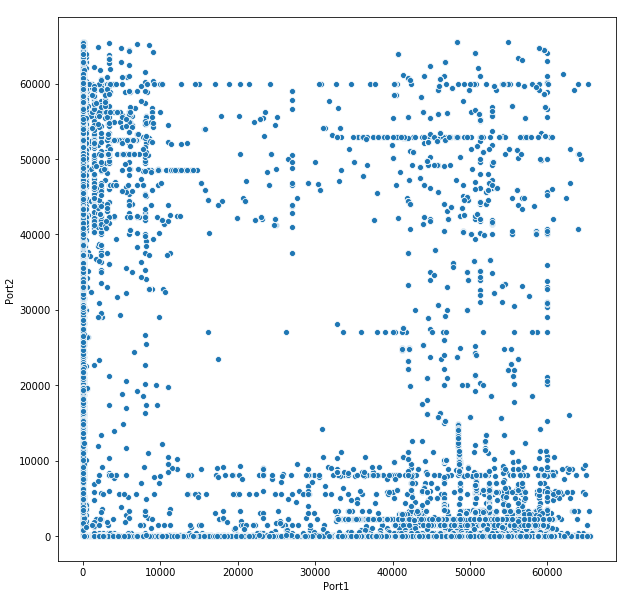
\includegraphics[width=0.8\linewidth]{figs/port1vs2.PNG}
     \caption{Gráfica de puntos entre puertos de origen y destino}
     \label{Fig:scatterport}
   \end{minipage}
\end{figure}

Utilizando las variables binarias como ejes, algunas demuestran cierta diferencia en la dispersión, como por ejemplo en las variables de número de puertos.

\begin{figure}[H]
   \begin{minipage}[b]{0.48\textwidth}
     \centering
     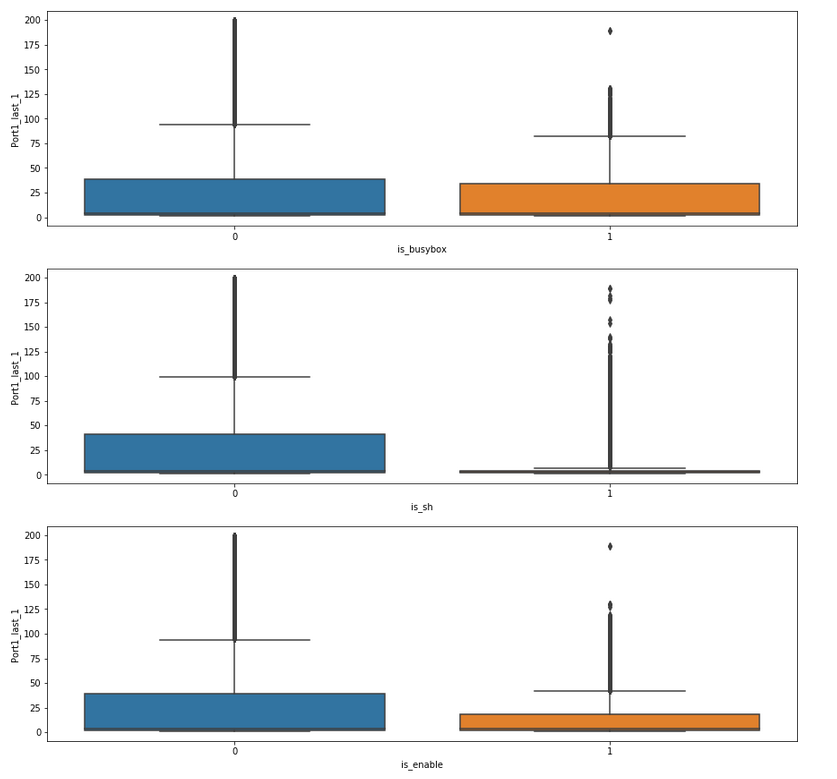
\includegraphics[width=0.8\linewidth]{figs/port1_bin.PNG}
     \caption{Diagramas de caja de número de puertos origen según variables binarias}
     \label{Fig:port1_bin}
   \end{minipage}\hfill
   \begin{minipage}[b]{0.48\textwidth}
     \centering
     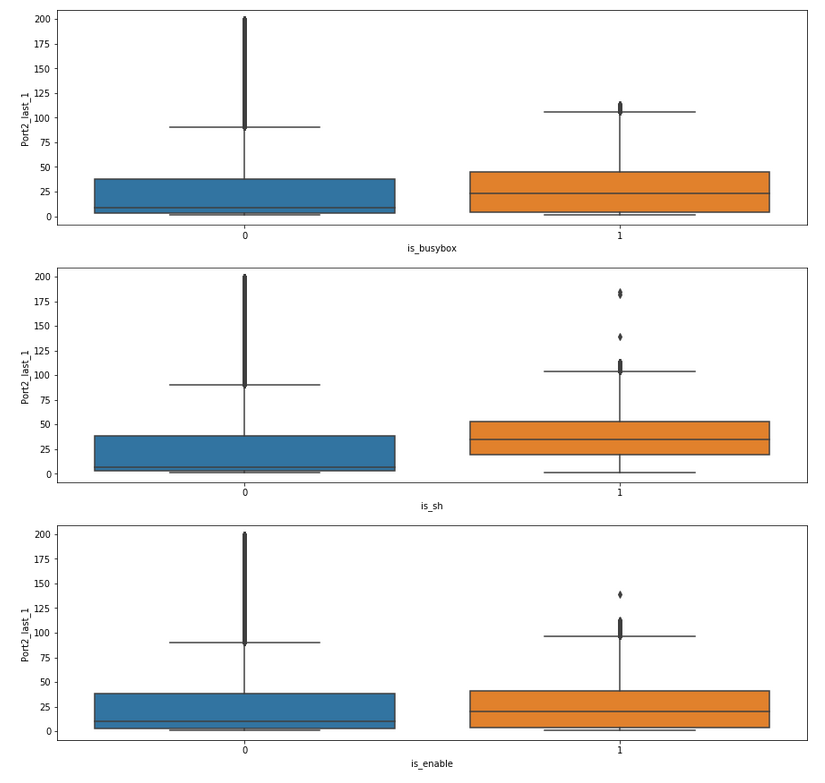
\includegraphics[width=0.8\linewidth]{figs/port2_bin.PNG}
     \caption{Diagramas de caja de número de puertos destino según variables binarias}
     \label{Fig:port2_bin}
   \end{minipage}
\end{figure}

\section{Creación del set de datos final}

Tal y como se ha comentado anteriormente, por lo general las conexiones realizadas en momentos anteriores no tienen por qué estar relacionadas entre sí, por lo que utilizar la marca de tiempo como índice de los datos para alimentar el modelo no acabaría siendo útil del todo. Por ello, se busca la forma de poder mantener una temporalidad dentro de las variables pero que las observaciones estén relacionadas según las conexiones de origen y destino.

La vía utilizada para generar este set de datos fue basarse en tomar las IPs como índice, es decir, una observación (fila) corresponde a una IP en la que las variables (columnas) tienen la temporalidad. Para ello se establecieron tres ventanas de tiempo distintos, 5 minutos, 10 minutos y 30 minutos, donde cada variable inicial genera nuevas variables como la media, suma, desviación típica y número de registros dentro del periodo total de conexiones (día dos de Febrero).

\begin{gather*}
n_{agregaciones} = 4 \\
n_{periodo} = \frac{T_{fin} - T_{ini}}{ventana} \\
n_{por variable} = n_{agregaciones} * n_{periodo} \\
total\_columnas = n_{por variable} * num\_variables
\end{gather*}

Según el tamaño de la ventana el \textit{dataset} resultante tendrá más o menos tamaño, debido a que una menor ventana implica la creación de más periodos en las variables. Por otro lado, no todas las conexiones tienen observaciones en los datos iniciales, es decir, hay conexiones que se pueden dar por la tarde y no por la mañana, para estas conexiones se rellena el valor a cero, por lo que si se observa la cantidad de ceros, se vera que se trata de una matriz dispersa. Un pequeño ejemplo del dataset resultante sería el siguiente:

\begin{figure}[h]
    \centering
    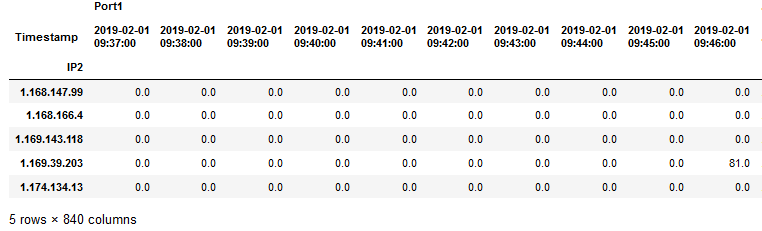
\includegraphics[width=16cm]{figs/dataset.PNG}
    \caption{Ejemplo de \textit{dataset} final}
    \label{fig:dataset}
\end{figure}

El \textit{dataset} tendrá las siguientes características (algunas visibles en \ref{fig:dataset}):
\begin{itemize}
    \item Las filas están formadas por las IPs.
    \item Se utilizan como índice las IPs únicas de origen y las IPs únicas de destino.
    \item Se diferencian mediante una variable binaria.
    \item La temporalidad se traslada a las columnas.
    \item Cada variable original se transforma en agregaciones durante el periodo total.
    \item La dimensionalidad del \textit{dataset} queda definida por la ventana de tiempo escogida.
    \item Una gran parte de los datos son ceros.
    \item La cantidad de filas es fija, dado que la cantidad única de IPs es constante independientemente de la ventana de tiempo.
\end{itemize}

Asimismo, sobre estas variables se podrían seguir generando nuevas variables utilizando distintas ventanas (\textit{rolling window}) sin embargo, para evitar aumentar el tamaño no se crearon nuevas ventanas. Por otro lado, se añadieron nuevas variables binarias indicando el valor de los últimos 8 bits, es decir, el host de las IPs. 

Se crearon varios datasets con el fin de identificar anomalías con distintas características, algunas pueden provenir de acciones muy rápidas en un tiempo pequeño que pueden ser detectadas por una ventana pequeña y aquellas acciones que se realicen periódicamente puedan ser detectadas por ventanas más largas.
\newpage

\section{Algoritmos de \textit{Machine Learning}}

Tras el estudio del estado del arte y las pruebas realizadas durante el preprocesamiento y la creación del \textit{dataset} la técnica utilizada es un ensamblado de dos algoritmos:
\begin{itemize}
    \item \textit{Isolation Forest}
    \item \textit{Autoencoder}
\end{itemize}

La decisión de realizar un ensamblado de varios modelos recae en la capacidad que otorga para generalizar mejor a la hora de realizar las detecciones y así evitar que ciertas observaciones puedan afectar en mayor medida al modelo.

\subsection{\textit{Isolation Forest}}

Como su nombre indica se trata de un modelo basado en árboles de decisión enfocado en el aislamiento de las observaciones. Este tipo de modelo funciona muy bien con \textit{datasets} de alta dimensionalidad y ofrece un rendimiento muy bueno dada su poca complejidad computacional y su bajo uso de memoria \cite{liu2008isolation}.

Mientras que la mayor parte de herramientas de detección de anomalías se basan en perfilar el uso normal de los casos y clasificar como anomalía aquello que diverja de este perfil, por ejemplo, una \textit{clusterización} podría indicar que un grupo no es anómalo debido al tamaño del mismo, además de hacer un uso mucho mayor de memoria debido al cálculo de las disimilitudes (o distancias). El \textit{Isolation Forest} se basa en otra metodología, donde en lugar de perfilar, pretende encontrar aquellas observaciones que más aisladas estén. Para ello se basa en dos premisas:
\begin{itemize}
    \item Las anomalías tienen atributos muy diferentes de los valores normales.
    \item La cantidad de anomalías presenta un porcentaje muy pequeño dentro de los datos.
\end{itemize}

En otras palabras, las anomalías son pocas y diferentes, por lo que son más propensas a estar aisladas que las observaciones normales. Este aislamiento se realiza mediante la creación de arboles de decisión, donde las anomalías necesitarán menos particiones para aislarse que los datos normales.

\begin{figure}[h]
    \centering
    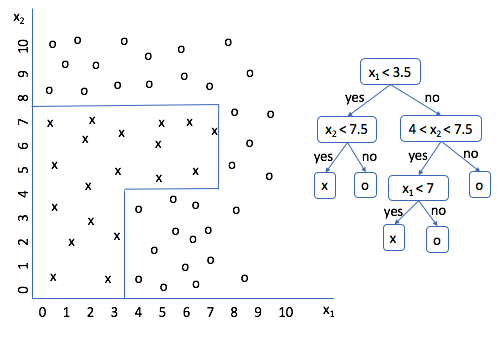
\includegraphics[width=10cm]{figs/tree.png}
    \caption{Fronteras en un árbol de decisión}
    \label{fig:tree_boundaries}
\end{figure}

La medida utilizada en el \textit{Isolation Forest} es la profundidad del árbol o \textit{path length}, por ejemplo la figura \ref{fig:tree_boundaries} tendría una profundidad de tres. Cada árbol realiza particiones aleatorias de modo que cada observación puede formar parte de varios árboles con distintas profundidades, por lo que el \textit{path length} final es la media de todos ellos. En la siguiente figura \ref{fig:isolation_forest} se observa como la primera observación ha necesitado de más particiones (más profundidad del árbol) para poder aislar la observación que el segundo caso, que ha necesitado de muchas menos, por ello este segundo punto tendrá una valoración más alta como anomalía.

\begin{figure}[h]
    \centering
    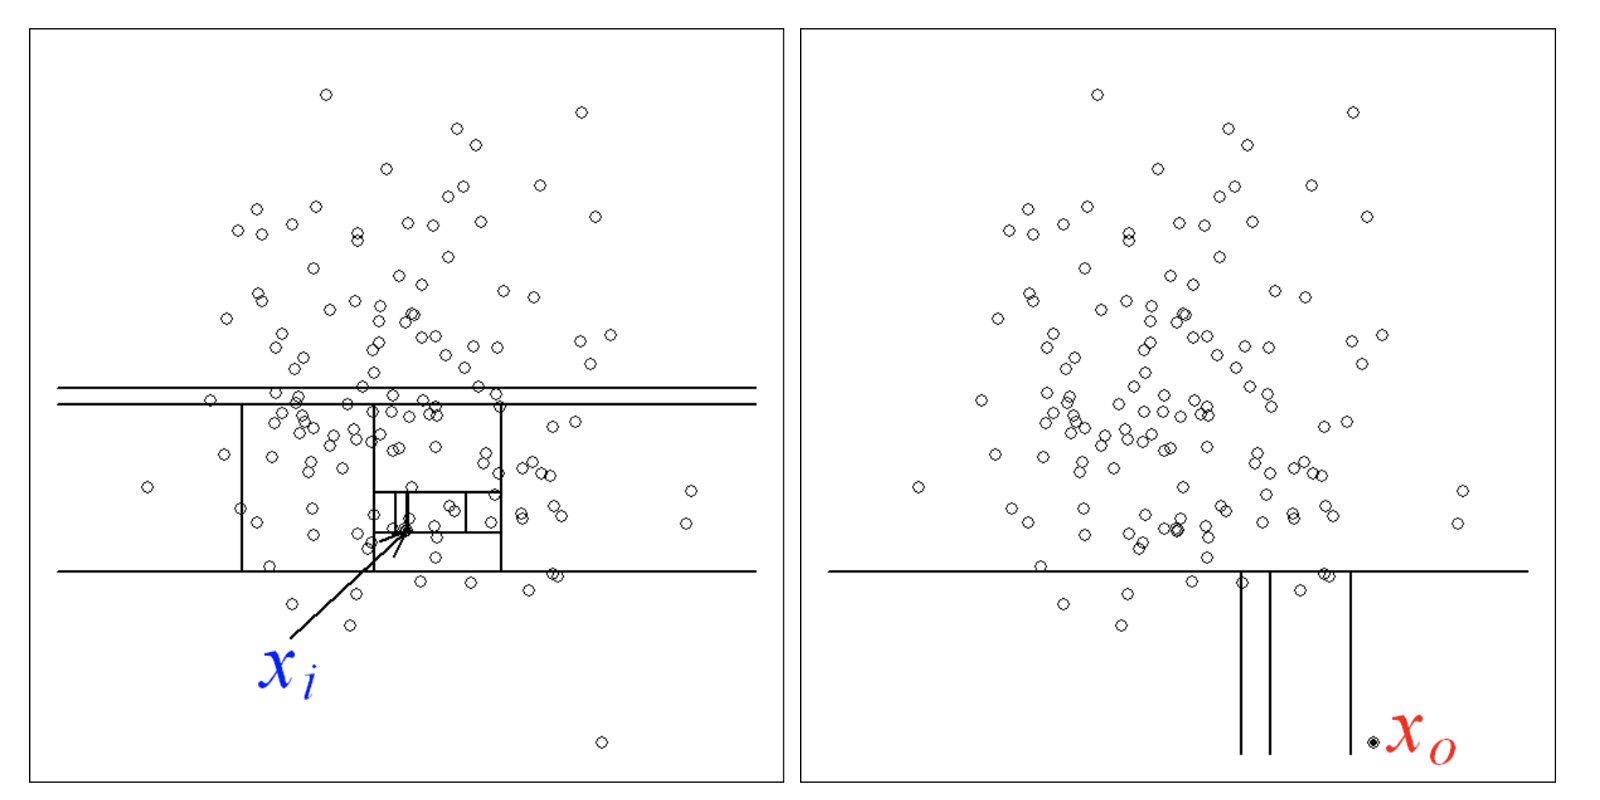
\includegraphics[width=12cm]{figs/isolation.png}
    \caption{Ejemplo de un árbol de \textit{Isolation Forest}}
    \label{fig:isolation_forest}
\end{figure}

Para la categorización como anomalía se define una puntuación que ayude a determinar que puntos pueden ser anómalos y cuales no. Tomando la profundidad de un árbol como \( h(x)\) y la media de profundidad como \( E(h(x))\) se puede definir una puntuación utilizando la profundidad estimada media \( c(n)\):

\begin{gather*}
c(n) = 2H(n-1) - (2(n-1)/n) \\
H(i) = ln(i) + 0.5772156649 \\
s(x,n) = 2^{-\frac{E(h(x))}{c(n)}} \\
\end{gather*}

Donde \textit{n} es el número de observaciones totales, \textit{x} una observación y \(s(x,n)\) la puntuación de anomalía. Los resultados de la puntuación se pueden interpretar de la siguiente manera según el cociente de \( c(n)\) y \( E(h(x))\):
\begin{itemize}
    \item Un valor cercano a uno, indica que se trato posiblemente de una anomalía.
    \item Un valor cercano a cero, indica que no es una anomalía.
    \item Si todas las observaciones devuelven un valor cercano a 0.5 se puede considerar que no existen anomalías.
\end{itemize}

Además de esta puntuación, para favorecer a la detección de anomalías, \textit{Isolation Forest} utiliza técnicas de submuestreo o \textit{subsampling} que favorece la identificación de las anomalías y disminuye el coste computacional.

\begin{figure}[h]
    \centering
    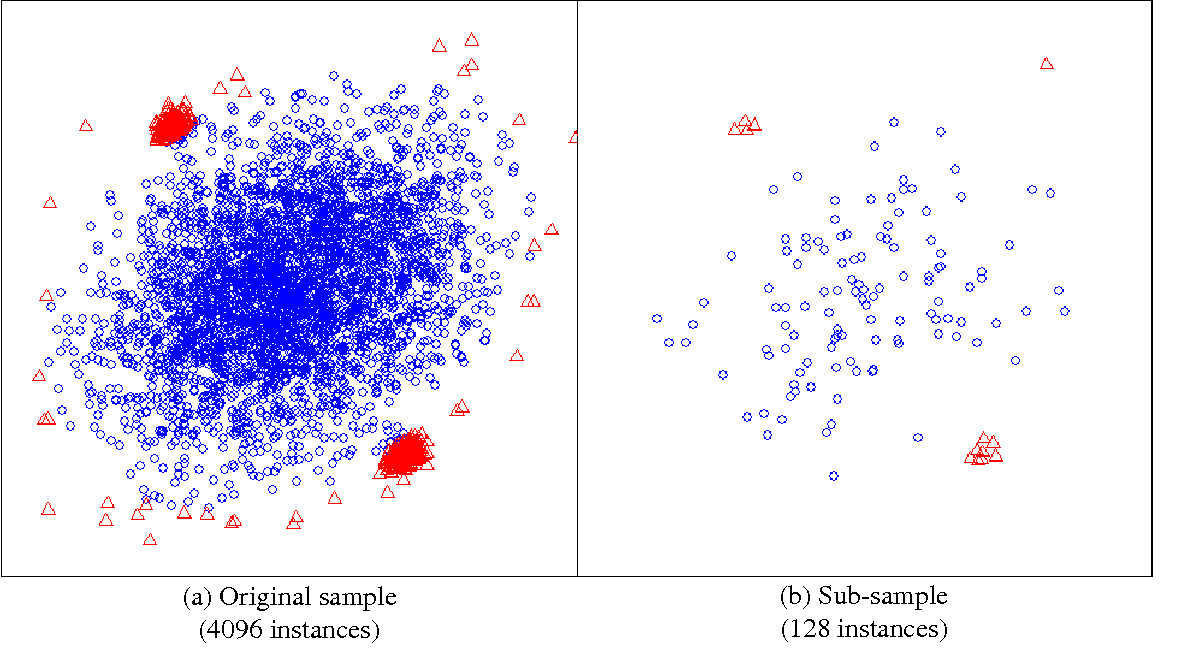
\includegraphics[width=10cm]{figs/subsample.png}
    \caption{Submuestreo aplicado en \textit{Isolation Forest}}
    \label{fig:subsample}
\end{figure}

\subsection{\textit{Autoencoder}}

El funcionamiento y características generales de los \textit{Autoencoders} se ha explicado en la sección \ref{subsubsection:Autoencoders}, por lo que en este apartado se explicará la arquitectura escogida.

Para este caso se ha construido un \textit{Deep Autoencoder}, es decir, varias capas ocultas que dependen de la cantidad de columnas de los datos de entrada, pero proporcionalmente mantiene la estructura. Consta de una capa de entrada, cinco capas intermedias (dos de \textit{Encoder}, dos de \textit{Decoder} y la representación de menor dimensionalidad) y una capa de salida.

Las dimensiones de las capas intermedias están definidas de la siguiente forma:
\begin{itemize}
    \item \textit{\(Encoder_1\) y \(Decoder_1\)}: \(\frac{ncol}{5}\)
    \item \textit{\(Encoder_2\) y \(Decoder_2\)}: \(\frac{ncol}{10}\)
    \item Representación: \(\frac{ncol}{25}\)
\end{itemize}

\begin{figure}[h]
    \centering
    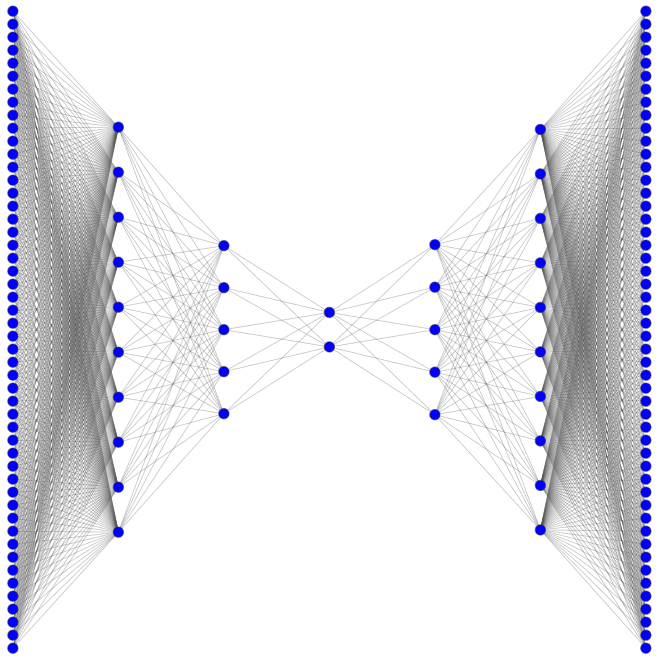
\includegraphics[width=10cm]{figs/ae_architecture.PNG}
    \caption{Arquitectura básica del \textit{Autoencoder}}
    \label{fig:ae_arch}
\end{figure}

Para la arquitectura anterior \ref{fig:ae_arch} se considera un \textit{dataset} con 50 columnas, por lo que la primera y penúltima capa tendrán 10 neuronas, las siguientes 5 neuronas y la capa central 2. El número de neuronas es proporcional al tamaño, por lo que crecerá acorde, redondeando hacia arriba para las divisiones no exactas.

Dado que el entrenamiento depende de la métrica de reconstrucción, esta se ha escogido acorde al tipo de datos con los que se entrena la red neuronal. Debido a las ventanas generadas y las agregaciones el tipo de variables resultantes son numéricas y en muy poca proporción por las variables de host hay 8 binarias, por ello la función de reconstrucción (o de pérdida para la red neuronal) utilizada es el error cuadrático medio \ref{eq:mse}.

\begin{equation}\label{eq:mse}
    MSE = \frac{1}{n}\sum_{t=1}^{n}X_i - \hat{X}
\end{equation}

Utilizando esta métrica, la red neuronal buscará disminuirlo lo máximo posible este error, aprendiendo de conexiones legítimas y anómalas. Aunque la red neuronal intente optimizar el error de estas últimas, se considera que la mayor parte de de las conexiones no son anómalas, por lo tanto la optimización en las anomalías no cobran tanto peso durante el entrenamiento y permiten diferenciarse del resto de puntos por el error de reconstrucción.

\subsection{Ensamblado de modelos}

Para el ensamblado de modelos se ha tomado como modelo "principal" el \textit{Isolation Forest}

% bibliografia
\addcontentsline{toc}{chapter}{Bibliografía}
\bibliographystyle{unsrt}
\bibliography{referencias}

\end{document}